% +----------------------------------------------+
% | Author: Jose Antonio Quinonero Gris          |
% | Creation date: Wednesday 20:44:47 22/11/2023 |
% +----------------------------------------------+
\documentclass[12pt, a4paper, final]{article}

% Basic configuration
\usepackage[utf8]{inputenc}
\usepackage[T1]{fontenc}
\usepackage{textcomp}
\usepackage{babel}
\usepackage{amsmath, amssymb}
% \usepackage{mathpazo} % mathpazo font
% \usepackage{achemso}

% Load custom configuration
%
% --- Formato de página ---
%
\usepackage[a4paper, top=2cm, bottom=2cm, left=2cm, right=2cm]{geometry}
\usepackage{lscape}
\usepackage{multicol}
\usepackage{fancyhdr}
\usepackage{titlesec}
% \pagestyle{fancy}
\usepackage{setspace}
% \singlespace      % Interlineado normal
% \onehalfspace       % Interlineado de 1.5
% \doublespace      % Interlineado doble
\spacing{1.3}     % Interlineado personalizado
% \renewcommand{\baselinestretch}{1.5} % Interlinieado de 1.5
\usepackage{afterpage}

\newcommand\blankpage{%
    \null
    \thispagestyle{empty}%
    \addtocounter{page}{-1}%
    \newpage}
% In the text before the blank page, insert the following code: \afterpage{\blankpage}
%
% --- Fuentes ---
%
%\usepackage[adobe-utopia]{mathdesign}
%\usepackage{mathspec}
\usepackage[many]{tcolorbox}   % for colored boxes
% \usepackage{setspace}   % for line spacing
%\usepackage{multicol}   % for multicolumns
%
% --- Redefinicion de entornos ---
%

%
% --- Copyright ---
%

%
% --- Figuras ---
%
\usepackage{graphicx}
\usepackage{import}
\usepackage{xifthen}
\pdfminorversion=7
\usepackage{pdfpages}
\usepackage{transparent}
\usepackage{xifthen}
\usepackage{calc}
% \usepackage{caption}
\usepackage{subcaption}
\usepackage{wrapfig}
\usepackage[margin=10pt,labelfont=bf]{caption}
\usepackage[bottom]{footmisc} % Para evitar que las figuras aparezcan por debajo del footnote
%
% --- Tablas ---
%
\usepackage{booktabs}
% \usepackage{tablefootnote}
\newcommand{\ra}[1]{\renewcommand{\arraystretch}{#1}} % Spacing btween lines of table
\usepackage{longtable}
\usepackage{array}
\usepackage{xtab}
\usepackage{multirow}
\usepackage{colortab}
\usepackage{bigdelim}
%
% -- Listas y estilo ---
%
\usepackage{enumerate}
\usepackage{enumitem}
%
% --- Matemáticas y física ---
%
\newcommand{\mat}[1]{\boldsymbol{\mathrm{#1}}}
% \decimalpoint
\usepackage{mathtools}
\usepackage{cancel} 
\usepackage[thinc]{esdiff}
\usepackage{physics}
\usepackage{braket}
\pdfsuppresswarningpagegroup=1
%
% --- Química ---
%
\usepackage{chemfig}
\usepackage{chemformula,array} % \ch{}
\usepackage[version=4]{mhchem}
\newcommand{\celsius}{$^{\circ}$C }
%
% --- Programming/Code ---
%
\usepackage{verbatimbox} % Centrar código con verbatim
%
% --- Referencias ---
%
\usepackage[colorlinks=true,
linkcolor = blue,
urlcolor  = blue,
citecolor = black,
anchorcolor = blue]{hyperref}
\usepackage{cleveref}
\newcommand{\equatref}[1]{eq.~(\ref{#1})}
\newcommand{\eqsref}[1]{Equations~(\ref{#1})}
\newcommand{\tabref}[1]{Table~\ref{#1}}
\newcommand{\figref}[1]{Figure~\ref{#1}}
%
% --- Otros ---
%
\usepackage{layouts}
% \printinunitsof{cm}\prntlen{\textwidth} % to print \textwidth in cm
\usepackage{rotating}
\usepackage{lipsum}
\usepackage{xcolor}
\usepackage[nottoc,numbib]{tocbibind}
\usepackage{blindtext}
\newcommand{\incfig}[1]{%
        \def\svgwidth{\columnwidth}
            \import{./figures/}{#1.pdf_tex}
        }
%
% --- Colores ---
%
\definecolor{blue1}{HTML}{5989cf}    % setting main color to be used
\definecolor{blue2}{HTML}{cde4ff}     % setting sub color to be used
\definecolor{mycyan}{HTML}{CBE5EA}     % setting sub color to be used
\definecolor{mycyan2}{HTML}{dcdde2}     % setting sub color to be used
\definecolor{mymint}{HTML}{DAF7A6}     % setting sub color to be used
%
% --- Cajas ---
%
\tcbuselibrary{many}   % many : loads the libraries skins, breakable, raster, hooks, theorems, fitting and xparse .
\newtcolorbox{bluebox}[2][]{
	tile,
	frame style={left color=red!75!black,right color=red!10!yellow},
	boxrule = 2pt,
    opacityfill = 1.0,
	arc is angular,
	fonttitle = \bfseries,
	title={#2}, #1
}
% Boxed equation
\usepackage{empheq}
\newtcbox{\mymathbox}[1][]{%
    nobeforeafter, math upper, tcbox raise base,
    standard jigsaw, sharp corners, colframe=white!45!black,
    colback=white!95!black, leftrule=4pt, rightrule=0pt, toprule=0pt, bottomrule=0pt,
    #1}
%
% --- Dedicatoria ---
%
\newenvironment{dedication}
{
   \cleardoublepage
   \thispagestyle{empty}
   \vspace*{\stretch{1}}
   \hfill\begin{minipage}[t]{0.66\textwidth}
   \raggedright
}%
{
   \end{minipage}
   \vspace*{\stretch{3}}
   \clearpage
}

% \newenvironment{dedication}
%   {\clearpage           % we want a new page
%    \thispagestyle{empty}% no header and footer
%    \vspace*{\stretch{1}}% some space at the top
%    \itshape             % the text is in italics
%    \raggedleft          % flush to the right margin
%   }
%   {\par % end the paragraph
%    \vspace{\stretch{3}} % space at bottom is three times that at the top
%    \clearpage           % finish off the page
%   }
%Clears plain-page pg# settings, relocates pg#'s @ top-right-corner.
\makeatletter
\renewcommand{\ps@plain}{
\renewcommand\@oddhead{\hfill\normalfont\textrm{\thepage}}
\renewcommand\@evenhead{}
\renewcommand\@oddfoot{}
\renewcommand\@evenfoot{}}
%
% --- Codigo ---
%
% \usepackage{minted}
\usepackage{listings}
\usepackage{lstautogobble}  % Fix relative indenting
\usepackage{zi4}            % Nice font

% =============================================================================
% AutoMultiColItemize
%
% Example:
% \begin{AutoMultiColItemize}
%   \item Item 1
%   \item Item 2
%   \item Item 3
%   \item Item 4
%   \item Item 5
%   \item Item 6
% \end{AutoMultiColItemize}
%
% It can be nested inside other itemize environments.
%
% Credit:
%   https://tex.stackexchange.com/questions/194426/split-itemize-into-multiple-columns
%   https://tex.stackexchange.com/questions/74595/count-and-use-the-number-of-items-in-advance
% -----------------------------------------------------------------------------
\newcounter{countitems}
\newcounter{nextitemizecount}
\newcommand{\setupcountitems}{%
  \stepcounter{nextitemizecount}%
  \setcounter{countitems}{0}%
  \preto\item{\stepcounter{countitems}}%
}
\makeatletter
\newcommand{\computecountitems}{%
  \edef\@currentlabel{\number\c@countitems}%
  \label{countitems@\number\numexpr\value{nextitemizecount}-1\relax}%
}
\newcommand{\nextitemizecount}{%
  \getrefnumber{countitems@\number\c@nextitemizecount}%
}
\newcommand{\previtemizecount}{%
  \getrefnumber{countitems@\number\numexpr\value{nextitemizecount}-1\relax}%
}
\makeatother    
\newenvironment{AutoMultiColItemize}{%
\ifnumcomp{\nextitemizecount}{>}{3}{\begin{multicols}{2}}{}%
\setupcountitems\begin{itemize}}%
{\end{itemize}%
\unskip\computecountitems\ifnumcomp{\previtemizecount}{>}{3}{\end{multicols}}{}}
% =============================================================================

% -----------------------------------------------------------------------------
% Otro estilo
% -----------------------------------------------------------------------------
\definecolor{bluekeywords}{rgb}{0.13, 0.13, 1}
\definecolor{greencomments}{rgb}{0, 0.5, 0}
\definecolor{redstrings}{rgb}{0.9, 0, 0}
\definecolor{graynumbers}{rgb}{0.5, 0.5, 0.5}

 \lstdefinestyle{otherStyle}{
    autogobble,
    columns=fullflexible,
    showspaces=false,
    showtabs=false,
    breaklines=true,
    showstringspaces=false,
    breakatwhitespace=true,
    escapeinside={(*@}{@*)},
    commentstyle=\color{greencomments},
    keywordstyle=\color{bluekeywords},
    stringstyle=\color{redstrings},
    numberstyle=\color{graynumbers},
    basicstyle=\ttfamily\footnotesize,
    frame=l,
    framesep=12pt,
    xleftmargin=12pt,
    tabsize=4,
    captionpos=b
}

% -----------------------------------------------------------------------------
% VS2017 C++ color scheme
% -----------------------------------------------------------------------------
\definecolor{clrbackground}{RGB}{255,255,255}
\definecolor{clrtext}{RGB}{0,0,0}
\definecolor{clrstring}{RGB}{163,21,21}
\definecolor{clrnamespace}{RGB}{0,0,0}
\definecolor{clrpreprocessor}{RGB}{128,128,128}
\definecolor{clrkeyword}{RGB}{0,0,255}
\definecolor{clrtype}{RGB}{43,145,175}
\definecolor{clrvariable}{RGB}{0,0,0}
\definecolor{clrconstant}{RGB}{111,0,138} % macro color
\definecolor{clrcomment}{RGB}{0,128,0}

\lstdefinestyle{VS}{
	backgroundcolor=\color{clrbackground},
	% basicstyle=\color{clrtext}, % any text
	basicstyle=\ttfamily\footnotesize\color{clrtext},
	stringstyle=\color{clrstring},
	identifierstyle=\color{clrvariable}, % just about anything that isn't a directive, comment, string or known type
	commentstyle=\color{clrcomment},
	% directivestyle=\color{clrpreprocessor}, % preprocessor commands
	% listings doesn't differentiate between types and keywords (e.g. int vs return)
	% use the user types color
	keywordstyle=\color{clrtype},
	% keywordstyle={[2]\color{clrconstant}}, % you'll need to define these or use a custom language
	tabsize=4
}

% -----------------------------------------------------------------------------
% Mi estilo
% -----------------------------------------------------------------------------
\definecolor{dkgreen}{rgb}{0,0.6,0}
\definecolor{gray}{rgb}{0.5,0.5,0.5}
\definecolor{mauve}{rgb}{0.58,0,0.82}

 \lstdefinestyle{myStyle}{
    frame=tb,
    captionpos=t,
    belowcaptionskip=0.5\baselineskip,
    breaklines=true,
    breakatwhitespace=true,
    columns=flexible,
    % frame=none,
    % numbers=none,
    numbers=left,
    numbersep=5pt,
    numberstyle=\tiny\color{gray},
    % basicstyle=\footnotesize\ttfamily,
    basicstyle=\footnotesize\sffamily,
    keywordstyle=\bfseries\color{green!40!black},
    % commentstyle=\itshape\color{white!40!black},
    commentstyle=\color{white!40!black},
    identifierstyle=\color{blue},
    stringstyle=\color{mauve},
    % backgroundcolor=\color{gray!20!white},
    backgroundcolor=\color{white},
    showspaces=false,
    showstringspaces=false,
    tabsize=4,
    showtabs=false,
    aboveskip=3mm,
    belowskip=3mm
}

 \lstdefinestyle{myStyle2}{
    frame=tb,
    captionpos=t,
    belowcaptionskip=0.5\baselineskip,
    breaklines=true,
    breakatwhitespace=true,
    % frame=none,
    numbers=left,
    numbersep=5pt,
    numberstyle=\tiny\color{gray},
    basicstyle=\ttfamily\footnotesize\color{clrtext},
    stringstyle=\color{clrstring},
    identifierstyle=\color{clrvariable}, % just about anything that isn't a directive, comment, string or known type
    commentstyle=\color{white!40!black},
    keywordstyle=\lst@ifdisplaystyle\color{clrtype}\fi,
    backgroundcolor=\color{clrbackground},
    showspaces=false,
    showstringspaces=false,
    tabsize=4,
    showtabs=false,
    aboveskip=3mm,
    belowskip=3mm
}

 \lstdefinestyle{inlinecode}{
    basicstyle=\ttfamily\color{clrtext},
    backgroundcolor=\color{clrbackground},
}
%
% =============================================================================
% Estilos disponibles:
%    - myStyle
%    - otherStyle
%    - VS2017
%
\lstset{style=myStyle2,language=bash}
\def\inline{\lstinline[basicstyle=\ttfamily,keywordstyle={},escapeinside={(*}{*)},mathescape=true]}

% \def\inline{\lstinline[basicstyle=\sffamily\color{black},keywordstyle={}]}
% \newcommand[1]{\inlinecode}{\textsf{#1}}

% \NewDocumentCommand{\code}{v}{%
% \textsf{#1}%
% }

% Document title and type
\newcommand{\doctitle}{Explorando el efecto túnel en la molécula de amoníaco} % The title of the thesis
\newcommand{\doctype}{Trabajo Fin de Grado}
% PhD Thesis
% Master's Thesis
% Bachelor's Thesis
% Thesis
% Dissertation
% End of Studies Project Report
% Graduation Project Report
% ...

% Info about university
\newcommand{\department}{Departamento de Química Física} % department
\newcommand{\degree}{Grado} % your degree (Licence, Bachelor, Applied Master, PhD, etc)
\newcommand{\major}{Química} % your major (Mathematics, Chemistry, Biology, etc)
\newcommand{\defenseDate}{Junio 2022} % defence date

% Thesis author
\newcommand{\authorName}{José Antonio Quiñonero Gris}

% Main supervisor
\newcommand{\supervisor}{José Zúñiga Román}

% Co-supervisor. If you have only one supervisor, leave it as it is
\newcommand{\cosupervisor}{Mr. Co-Supervisor's Name}

% Committee members
\newcommand{\tribunalI}{Persona x}
\newcommand{\tribunalII}{Persona y}
\newcommand{\tribunalIII}{Persona z}
% \newcommand{\reviewer}{Ms. Reviewer's Name}
% \newcommand{\secondReviewer}{Mr. Second Reviewer's Name}
% \newcommand{\thirdReviewer}{Mr. Third Reviewer's Name}

% Dates. Default to current current date.
\newcommand{\Year}{\the\year{}}

% Signature date (defaults to today).
\newcommand{\signatureDate}{\ddmmyyyydate\today}

% PDF Metadata
\newcommand{\keywords}{Tunneling, Quantum Mechanics, Ammonia}

\newcommand{\university}{Universidad de Murcia}
\newcommand{\school}{Facultad de Química}

% PDF settings
\hypersetup
{
    pdfauthor={\authorName},
    pdfsubject={\doctitle},
    pdfkeywords={\keywords}
}

\newcommand{\fordm}{$D^{(1)}$}
\newcommand{\sordm}{$D^{(2)}$}

\newcommand{\nota}[1]{\textcolor{red}{#1}}

% \usepackage[backend=biber,style=chem-acs,terseinits=true,sorting=none,isbn=false,doi=false]{biblatex}
% \addbibresource{/home/jose/Documents/latex/preamble/references} % extension must be written
%%%%
\usepackage[backend=bibtex,style=chem-acs,terseinits=true,sorting=none,isbn=false,doi=false]{biblatex}
% \usepackage[backend=bibtex,style=chem-acs,terseinits=true,sorting=none,isbn=false,doi=false]{biblatex}
\bibliography{/home/jose/Documents/latex/preamble/references}
%%%
\ExecuteBibliographyOptions{%
  citetracker=true,% Citation tracker enabled in order not to repeat citations, and have two lists.
  sorting=none,% Don't sort, just print in the order of citation
  alldates=long,% Long dates, so we can tweak them at will afterwards
  dateabbrev=false,% Remove abbreviations in dates, for same reason as ``alldates=long''
  articletitle=true,% To have article titles in full bibliography
  maxcitenames=999% Number of names before replacing with et al. Here, everyone.
  }

% No brackets around the number of each bibliography entry
\DeclareFieldFormat{labelnumberwidth}{#1\addperiod}

% Suppress article title, doi, url, etc. in citations
\AtEveryCitekey{%
  \ifentrytype{article}
    {\clearfield{title}}
    {}%
  \clearfield{doi}%
  \clearfield{url}%
  \clearlist{publisher}%
  \clearlist{location}%
  \clearfield{note}%
}

% Print year instead of date, when available; make use of urldate
\DeclareFieldFormat{urldate}{\bibstring{urlseen}\space#1}
\renewbibmacro*{date}{% Based on date bib macro from chem-acs.bbx
  \iffieldundef{year}
    {\ifentrytype{online}
       {\printtext[urldate]{\printurldate}}
       {\printtext[date]{\printdate}}}
    {\printfield[date]{year}}}

% Remove period from titles
\DeclareFieldFormat*{title}{#1}
% Make year bold for @book types
\DeclareFieldFormat[book]{date}{\textbf{#1}} % doctorate added this line
\DeclareFieldFormat[book]{title}{\textit{#1}} % doctorate added this line
\DeclareFieldFormat[book]{publisher}{#1,} % doctorate added this line
% Embed doi and url in titles, when available
\renewbibmacro*{title}{% Based on title bib macro from biblatex.def
  \ifboolexpr{ test {\iffieldundef{title}}
               and test {\iffieldundef{subtitle}} }
    {}
    {\ifboolexpr{ test {\ifhyperref}
                  and not test {\iffieldundef{doi}} }
       {\href{http://dx.doi.org/\thefield{doi}}
          {\printtext[title]{%
             \printfield[titlecase]{title}%
             \setunit{\subtitlepunct}%
             \printfield[titlecase]{subtitle}}}}
       {\ifboolexpr{ test {\ifhyperref}
                     and not test {\iffieldundef{url}} }
         {\href{\thefield{url}}
            {\printtext[title]{%
               \printfield[titlecase]{title}%
               \setunit{\subtitlepunct}%
               \printfield[titlecase]{subtitle}}}}
         {\printtext[title]{%
            \printfield[titlecase]{title}%
            \setunit{\subtitlepunct}%
            \printfield[titlecase]{subtitle}}}}%
     \newunit}%
  \printfield{titleaddon}%
  \clearfield{doi}%
  \clearfield{url}%
  \clearfield{pagetotal}%
  \clearlist{language}% doctorate added this
  \clearfield{note}% doctorate added this
  \ifentrytype{article}% Delimit article and journal titles with a period
    {\adddot}
    {}}

\newcommand{\ttitle}{New parametrization of the Second-order Reduced Density Matrix (2-RDDM)}
\newcommand{\stitle}{\large{Subtitle}}
\newcommand{\finaldate}{\today}
\newcommand{\authorname}{José Antonio \textsc{Quiñonero Gris}}
\newcommand{\univname}{Máster Erasmus Mundus en Química Teórica y Modelización Computacional}
\newcommand{\worktype}{Trabajo Fin de Máster}
\newcommand{\supname}{Alfredo \textsc{Sánchez de-Merás}}
\newcommand{\degreename}{The degree}
\newcommand{\deptname}{Departamento de Química Física}
\newcommand{\facultyname}{Universitat de Valencia}
\newcommand{\institutename}{Facultad de Química}
\newcommand{\centername}{Center name}
\newcommand{\kkeywords}{keyword1, keyword2}
\newcommand{\HRule}{\rule{.9\linewidth}{.6pt}} % New command to make the lines in the title page


\usepackage{./configuration/mybraket}

\spacing{1.15}     % Interlineado personalizado

% =============================================================================
%                             --- Other information ---
% =============================================================================
\bibliography{./TFM}

\graphicspath{{./figures/}}

% Default title in case the front page is not used
\author{\authorname}
\title{
    \vspace{-2cm}
    \textbf{\ttitle}
}

\hypersetup{
pdfauthor={\authorname},
pdftitle={\ttitle},
pdfsubject={},
pdfkeywords={\kkeywords}
}

\date{\today}

%%%%%%%%%%%%%%%%%%%%%%%%%%%%%%%%%%%%%%%%%%%%%%%%%%%%%%%%%%%%%%%%%%%%%%%%%%%%%%%
\begin{document}
% =============================================================================
%                             --- Title ---
% =============================================================================
%
% Possible options:
%
% 1) Simple title in the same page
%
% \maketitle
%
% 2) Simple title with more info in the same page
%
% \thispagestyle{empty}
% \begin{center}
    {\bfseries\large \univname \par}
    \vspace{0.1cm}
    {\scshape\large \facultyname \par}
    \vspace{0.5cm}
    {\bfseries\scshape\Large \ttitle \par}
    \vspace{0.5cm}
    % {\itshape\Large \worktype \par}
    % \vfill
    % {\Large Author: \par}
    {\large \authorname \par}
    % \vfill
    {\large \finaldate \par}
\end{center}

%
% 4) Simple title but in a separate page
%
% \thispagestyle{empty}
% \maketitle
%
% 4) A minimal titlepage
%
% \afterpage{\blankpage}
% \begin{titlepage}
    \centering
    {\bfseries\LARGE \univname \par}
    \vspace{1cm}
    {\scshape\Large \facultyname \par}
    \vspace{3cm}
    {\scshape\Huge \ttitle \par}
    \vspace{3cm}
    {\itshape\Large \worktype \par}
    \vfill
    {\Large Author: \par}
    {\Large \authorname \par}
    \vfill
    {\Large \finaldate \par}
\end{titlepage} 
\clearpage
%
% 5) A more elaborated titlepage
%
% \graphicspath{{./front-page/figures/}}
% \thispagestyle{empty}
\begin{titlepage}
\begin{center}

% \vspace*{.06\textheight}
\vfill

\includegraphics[width=0.3\textwidth]{escudo.pdf}\\[0.2cm]
{\scshape\LARGE \univname\par}\vspace{0.3cm} % University name
\textsc{\Large \facultyname}\\[0.3cm] % Thesis type
\Large \worktype\\ [0.2cm]

\HRule \\[0.4cm] % Horizontal line
{\Large \bfseries \ttitle\par}\vspace{0.4cm} % Thesis title
\HRule \\[0.5cm] % Horizontal line

\begin{minipage}[t]{0.4\textwidth}
\begin{flushleft} \large
\emph{Autor:}\\
\authorname % Author name - remove the \href bracket to remove the link
\end{flushleft}
\end{minipage}
\begin{minipage}[t]{0.4\textwidth}
\begin{flushright} \large
\emph{Tutor:} \\
\supname % Supervisor name - remove the \href bracket to remove the link
\end{flushright}
\end{minipage}\\[1.5cm]

\vfill

%\large \textit{A thesis submitted in fulfillment of the requirements\\ for the degree of %\degreename}\\[0.3cm] % University requirement text
%\textit{in the}\\[0.4cm]
%\groupname\\\deptname\\[2cm] % Research group name and department name

\large
\deptname\\[0cm] % Research group name and department name
\institutename\\[0cm] % University requirement text
% \centername\\[0cm] % University requirement text

% \vfill

{\large Julio - Agosto de 2022}\\[4cm] % Date

\vfill
\end{center}
\end{titlepage}
\afterpage{\blankpage}
\afterpage{\blankpage}\graphicspath{{./front-page/figures/}}
% \thispagestyle{empty}
\begin{titlepage}
\begin{center}

% \vspace*{.06\textheight}
\vfill

\includegraphics[width=0.3\textwidth]{escudo.pdf}\\[0.2cm]
{\scshape\LARGE \univname\par}\vspace{0.3cm} % University name
\textsc{\Large \facultyname}\\[0.3cm] % Thesis type
\Large \worktype\\ [0.2cm]

\HRule \\[0.4cm] % Horizontal line
{\Large \bfseries \ttitle\par}\vspace{0.4cm} % Thesis title
\HRule \\[0.5cm] % Horizontal line

\begin{minipage}[t]{0.4\textwidth}
\begin{flushleft} \large
\emph{Autor:}\\
\authorname % Author name - remove the \href bracket to remove the link
\end{flushleft}
\end{minipage}
\begin{minipage}[t]{0.4\textwidth}
\begin{flushright} \large
\emph{Tutor:} \\
\supname % Supervisor name - remove the \href bracket to remove the link
\end{flushright}
\end{minipage}\\[1.5cm]

\vfill

%\large \textit{A thesis submitted in fulfillment of the requirements\\ for the degree of %\degreename}\\[0.3cm] % University requirement text
%\textit{in the}\\[0.4cm]
%\groupname\\\deptname\\[2cm] % Research group name and department name

\large
\deptname\\[0cm] % Research group name and department name
\institutename\\[0cm] % University requirement text
% \centername\\[0cm] % University requirement text

% \vfill

{\large Julio - Agosto de 2022}\\[4cm] % Date

\vfill
\end{center}
\end{titlepage}

%
% =============================================================================
%                             --- Main text ---
% =============================================================================
\pagenumbering{Roman}  % Cambia a numeración romana
\setcounter{page}{1}    % Reinicia la numeración de página a 1
% ------
\section*{Abstract}
% ------
In this thesis, the application of Reduced Density Matrix 
Functional Theory (RDMFT) in the context of electronic structure calculations
is explored.
Therefore, the viability and 
accuracy of using one-particle (1-RDM) and two-particle reduced density 
matrices (2-RDM) in place of traditional wavefunction methods is investigated.
Both exact RDMs, computed from the integration of the wavefunction, and
approximated RDMs are studied.
The primary objective is to create a working environment that 
enables the optimization and verification of a potentially new parametrization
of the 2-RDM proposed by our group and explained within this document.

A significant advantage of RDMFT over conventional wavefunction-based methods 
is its ability to handle static correlation effects efficiently, making it a 
promising approach for systems where these effects are pronounced.
Additionally, the use of reduced density matrices simplifies the treatment of 
the kinetic energy term and avoids the need for introducing a fictitious non-interacting
system, as required in Density Functional Theory (DFT).

Despite its potential, the application of RDMFT is currently limited to small 
systems due to the computational complexity associated with larger systems.
This limitation stems from the intricate nature of constructing and managing 
higher-order density matrices and the challenges in ensuring their $N$-representability.

Future research directions include extending the methodologies proposed in 
this thesis to Time-Dependent Reduced Density Matrix Functional Theory (TDRDMFT),
which would enable the study of dynamic processes in electronic systems.
Moreover, significant theoretical advancements have been made over the past 
decades, particularly with the development of contracted Schrödinger equations 
and higher-order reduced density matrices, which promise to 
further enhance the applicability and robustness of RDMFT.

In conclusion, this work provides a comprehensive framework for employing 
RDMFT in electronic structure calculations, demonstrating its potential 
advantages and outlining the challenges that need to be addressed for broader application.

\vspace{0.3cm}
\textbf{Objectives:}
\begin{enumerate}[label={}]
    \item \textit{First:} Create a program integrated with the Dalton software for the computation
        of exact RDMs
    \item \textit{Second:} Validate available approximations for the electron repulsion functional
        in terms of the 2-RDM.
    \item \textit{Third:} Develop the formalism of a possible new approximation and propose possible
        parametrization and optimization methods.
    \item \textit{Fourth:} Create a framework for the construction, testing and deeper study of
        the 2-RDM, with the computation of RDM-derived properties, as the energy,
        comparable with the literature and/or software calculations, and
        direct metrics, as the Minkowski distance, for the direct comparison
        of RDMs.
\end{enumerate}
 \clearpage
% ------
\section*{Resumen}
% ------
En este Trabajo Fin de Máster, la aplicación de la Teoría del Funcional de la
Matriz de Densidad Reducida (RDMFT, por sus siglas en inglés) en el contexto de
los cálculos de estructura electrónica es explorada.
Se estudia la viabilidad y precisión resultantes del uso de las
matrices densidad reducidas de primer orden (1-RDM) y segundo orden (2-RDM)
en lugar de la función de onda en los métodos tradicionales.
Tanto las RDMs exactas, calculadas a partir de su definición formal, como 
distintas RDMs aproximadas son estudiadas.
El objetivo es crear un entorno de trabajo que permita la optimización y 
verificación de una potencialmente nueva parametrización de la 2-RDM propuesta
por nuestro grupo y desarrollada en este documento.

% Una ventaja significativa de la RDMFT frente a los métodos convencionales
% basados en la función de onda es la eficiencia con la que los efectos de
% correlación estáticos son considerados, haciendo a la RDMFT una teoría prometedora
% en el tratamiento de sistemas con efectos de correlación estática notables.
Una ventaja significativa de la RDMFT frente a los métodos convencionales
basados en la función de onda es su capacidad para manejar eficazmente los 
efectos de correlación estática, lo que la convierte en un enfoque prometedor 
para sistemas donde estos efectos son pronunciados.
Además, el  uso de RDMs simplifica el tratamiento
del término de energía cinética y evita la necesidad de introducir un
sistema ficticio no-interactuante, como se requiere en la Teoría del Funcional de la
Densidad (DFT).

A pesar de su potencial, la aplicación de la RDMFT está actualmente limitada a 
sistemas pequeños debido a su complejidad computacional.
Esta limitación se deriva de la naturaleza compleja
de las RDMs de orden superior y de garantizar su
$N$-representabilidad.

Futuras líneas de investigación incluyen extender estas metodologías 
a la Teoría del Funcional de la Matriz de Densidad 
Reducida Dependiente del Tiempo (TDRDMFT), lo que 
permitiría el estudio de procesos dinámicos en sistemas electrónicos.
Además, se han realizado avances teóricos significativos en las últimas décadas,
particularmente con el desarrollo de las ecuaciones de Schrödinger contraídas y 
RDMs de orden superior, que prometen mejorar aún más 
la aplicabilidad y robustez de la RDMFT.

En conclusión, este trabajo proporciona un marco comprensivo para emplear la 
RDMFT en cálculos de estructura electrónica, demostrando sus ventajas 
y desafíos que deben abordarse para una aplicación más amplia.

\vspace{0.3cm}
\textbf{Objetivos:}
\begin{enumerate}[label={}]
    \item \textit{Primero:} Crear un programa integrado con el software Dalton 
        para la obtención de RDMs exactas.
    \item \textit{Segundo:} Validar algunas de las aproximaciones disponibles
        para el funcional de repulsión electrónica en términos de la 2-RDM.
    \item \textit{Tercero:} Desarrollar la hipótesis de una posible nueva 
        aproximación y proponer posibles métodos de parametrización y optimización.
    \item \textit{Cuarto:} Crear un entorno de trabajo para la construcción, prueba y 
        estudio profundo de la 2-RDM, con el cálculo de propiedades derivadas 
        de la RDM, como la energía, comparables con la literatura y/o otros cálculos, 
        y métricas directas, como la distancia de Minkowski, para 
        la comparación directa de RDMs.
\end{enumerate}

 \clearpage
\tableofcontents \clearpage
% ------
\section*{List of Acronyms}
% ------

\begin{itemize}
    \item 1-RDM: One-particle Reduced Density Matrix
    \item 2-RDM: Two-particle Reduced Density Matrix
    \item AO: Atomic Orbital
    \item BB: Buijse-Baerends
    \item CAS: Complete Active Space
    \item CASSCF: Complete Active Space Self-Consistent Field
    \item DFT: Density Functional Theory
    \item DMF: Density Matrix Functional
    \item FCI: Full Configuration Interaction
    \item HF: Hartree-Fock
    \item HOSVD: Higher-order Singular Value Decomposition
    \item LS: Löwdin-Shull
    \item MO: Molecular Orbital
    \item MP2: Møller-Plesset perturbation theory of second order
    \item NEPOLD: A keyword in Dalton software related to the wave functions
    \item NOF: Natural Orbital Functional
    \item ON: Occupation Number
    \item RDM: Reduced Density Matrix
    \item RDMFT: Reduced Density Matrix Functional Theory
    \item SCF: Self-Consistent Field
    \item SDP: Semidefinite Programming
    \item SVD: Singular Value Decomposition
    \item TDRDMFT: Time-Dependent Reduced Density Matrix Functional Theory
\end{itemize}
 \clearpage
\pagenumbering{arabic}  % Cambia a numeración arábiga
\setcounter{page}{1}    % Reinicia la numeración de página a 1
\graphicspath{{./figures/}}

% ------
\section{Introduction}
% ------
Second quantization formalism is used in the document. 
Consequently, some useful definitions\mycite{helgaker2000second} are recalled
in \cref{sec:second-quantization}.

Also, Dirac (braket) notation is mainly used in the document except for 
\cref{sec:methodology-calculations}, where the Mulliken (chemistry) notation
is used.

The two-electron integrals are given, in Dirac notation, by 
\begin{equation} \label{eq:dirac-notation}
    \Braket{pq | rs} =
    \iint 
    \psi_p^{*} \left( \mat{r}_1 \right)
    \psi_q^{*} \left( \mat{r}_2 \right)
    \frac{1}{\left| \mat{r}_1 - \mat{r}_2 \right|}
    \psi_r \left( \mat{r}_1 \right)
    \psi_s \left( \mat{r}_2 \right)
    \dd{ \mat{r}_1} \dd{ \mat{r}_2}
    ,
\end{equation}
and in Mulliken notation by
\begin{equation} \label{eq:mulliken-notation}
    \PBraket{pq | rs} =
    \iint 
    \psi_p^{*} \left( \mat{r}_1 \right)
    \psi_q     \left( \mat{r}_1 \right)
    \frac{1}{\left| \mat{r}_1 - \mat{r}_2 \right|}
    \psi_r^{*} \left( \mat{r}_2 \right)
    \psi_s     \left( \mat{r}_2 \right)
    \dd{ \mat{r}_1} \dd{ \mat{r}_2}
    ,
\end{equation}
with the equivalence 
\begin{equation} \label{eq:dirac-mulliken-equivalence}
    \Braket{pq | rs} = \PBraket{pr | qs}
    .
\end{equation}

Additionally, atomic units are used all throughout the document.

\subsection{Reduced Density Matrix Functional Theory} % (fold)

% subsubsection 1-RDM (end)
Many methods of electronic structure theory are based on variational
optimization of an energy functional.
An idempotent first-order reduced density matrix (1-RDM) is variationally
optimized in the Hartree-Fock (HF) method\mycite{kollmar2004structure}.

The 1-RDM is determined by the natural orbitals and their occupation
numbers\mycite{lowdin1955quantuma}, leading to denote the corresponding energy
functional as density matrix functional (DMF) or natural orbital functional (NOF).
This is explained in detail in the following sections.

% \subsubsection{1-RDM} % (fold)
% \label{sec:1-RDM}

% subsubsection 1-RDM (end)
% NOTAS SACADAS DEL PERNAL
% mirar tb seccion 1.7.3 del Hergakel
In the coordinate representation of first quantization,
the \textit{first-order reduced density matrix} (1-RDM), $\fordm$, is defined
for an $n$-electron wavefunction, $\Psi$, as
\begin{equation} \label{eq:fordm-coordinate-representation}
    \fordm \left( \mat{x}_1, \mat{x}_1\myprime \right) =
    n \idotsint
    \Psi \left( \mat{x}_1, \mat{x_2}, \ldots,  \mat{x}_n \right)
    \Psi^{*} \left( \mat{x}_1\myprime, \mat{x_2}, \ldots,  \mat{x}_n \right)
    \dd{ \mat{x}_2} \cdots \dd{ \mat{x}_n}
    ,
\end{equation}
and the \textit{second-order reduced density matrix} (2-RDM), $\sordm$, as 
\begin{equation} \label{eq:sordm-coordinate-representation}
    \sordm \left( \mat{x}_1, \mat{x}_2, \mat{x}_1\myprime, \mat{x}_2\myprime \right)
    =
    \frac{n\left( n - 1 \right)}{2} \idotsint
    \Psi \left( \mat{x}_1, \mat{x}_2, \mat{x}_3, \ldots,  \mat{x}_n \right)
    \Psi^{*} \left( \mat{x}_1\myprime, \mat{x}_2\myprime, \mat{x}_3, \ldots,  \mat{x}_n \right)
    \dd{ \mat{x}_3} \cdots \dd{ \mat{x}_n}
    ,
\end{equation}
where $ \mat{x} = \left( \mat{r}, s \right)$ is a combined spatial and spin
coordinate.

%TODO: incluir info de seccion 2 del pernal

% An inmidiate advantage of using 1-RDM instead of the electron density, $\rho$,
% is that the kinetic energy is an explicit functional of $\fordm$ but not of
% $\rho$.
Employing the 1-RDM rather than the electron density, $\rho$, has the immediate
advantage of making the kinetic energy an explicit functional of $\fordm$ rather
than $\rho$.

% Then, there is no need to introduce a ficticious noninteracting system.
Then, introducing a fictitious noninteracting system is not necessary.

% Moreover, orbitals present in Reduced Density Matrix Functional Theory (RDMFT)
% are fractionally occupied, so functionals 
% of $\fordm$ seem to be better suited to account for static correlation.
Furthermore, fractionally occupied orbitals are a feature of Reduced Density 
Matrix Functional Theory (RDMFT), which suggests that functionals of $\fordm$ are 
better suited to explain static correlation.

Self-adjointness of $\fordm$, as defined in \cref{eq:fordm-coordinate-representation},
allows for its spectral representation\mycite{lowdin1955quantum}
\begin{equation}
    \fordm \left( \mat{x}, \mat{x}\myprime \right) =
    \sum_{p} n_p 
    \varphi_p \left( \mat{x} \right)
    \varphi_p^{*} \left( \mat{x}\myprime \right)
    .
\end{equation}

The eigenvalues of 1-RDM are called natural occupation numbers,
$\left\{ n_p \right\}$, and the eigenfunctions are known as natural
spin-orbitals, $\left\{ \varphi_p \right\}$.
% For convention, the indices $p,q,r,s$ are referred to natural spin-orbitals
% and $a,b,c,d$ to arbitrary one-eletron functions.
% Also, atomic units are employed throughout the document.
By convention, natural spin-orbitals are denoted by the indices $p$, $q$, $r$, and $s$, 
and arbitrary one-eletron functions by the indices $a$, $b$, $c$, and $d$. 

% Some properties of the natural spin-orbitals and occupation numbers, known as the 
% $n$-representability conditions, are:
% the ensemble n-representability conditions for the first-order reduced density
% matrix have a particularly simple form\mycite{coleman1963structure}
The ensemble $n$-representability conditions, which are some properties of the 
natural spin-orbitals and occupation numbers, have a particularly simple 
form\mycite{coleman1963structure} and read:
\begin{enumerate}
    \item Self-adjointness of $\fordm$: implies orthonormality of the natural orbitals 
        \begin{equation} \label{ec:self-adjoint-condition}
            \int
            \varphi_p^{*} \left( \mat{x} \right)
            \varphi_q \left( \mat{x} \right)
            = \delta_{pq}
            \quad \forall_{p,q} 
            .
        \end{equation}
        
    \item By the Löwdin's normalization convention\mycite{lowdin1955quantum},
        $\fordm$ is assumed to be normalized to a number of electrons, $n$.
        Therefore, the natural occupancies sum up to $n$  
        \begin{equation} \label{ec:normalization-condition}
            \trace \left[ \fordm \right] =
            \sum_{p} \fordm_{pp} =
            \sum_{p} n_p =
            n
            .
        \end{equation}

    \item Occupation number, $n_p$, is nonnegative and not grater than 1 
    \begin{equation} \label{ec:occ-number-condition}
        0 \leq n_p \leq 1 \quad \forall_{p}
        .
    \end{equation}
\end{enumerate}


\subsection{Properties in terms of the density matrices} % (fold)
\label{sub:Properties in terms of the density matrices}

% subsection Properties in terms of the density matrices (end)
% As demonstrated by Gilbert, who extended the Hohenberg-Kohn theorems to nonlocal
% potentials\mycite{gilbert1975hohenbergkohn, donnelly1978elementary}, there
% exists a 1-RDM functional\mycite{gilbert1975hohenbergkohn, hohenberg1964inhomogeneousa}
% such that
Gilbert theorem\mycite{gilbert1975hohenbergkohn} states that the expectation
value of any observable of a system in its ground state is a unique functional
of the ground-state 1-RDM, establishing the 1-RDM as the fundamental quantity
in RDMFT in place of the electronic density on which density functional theory
(DFT) is based.
It has been proved that there is a 1-RDM functional\mycite{gilbert1975hohenbergkohn, hohenberg1964inhomogeneousa}
such that the Hohenberg-Kohn theorems is extended to 
nonlocal potentials\mycite{gilbert1975hohenbergkohn, donnelly1978elementary}
\begin{equation} \label{ec:HK-functional}
    \func{E_{\nu}^{\text{HK}}}{\fordm} = 
    \mytrace{\hat{h} \hat{\fordm}} + 
    \Braket{\func{\Psi}{\fordm} | \hat{V}_{\text{ee}} | \func{\Psi}{\fordm}}
    ,
\end{equation}
% where $\func{\Psi}{\fordm}$ denotes a ground state wavefunction pertinent to a
% $\nu$-representable $\fordm$.
% $\hat{h}$ stands for a one-electron Hamiltonian comprising the kinetic
% energy, $\hat{T}$, and external potential, $\hat{V}_{\text{ext}}$ 
where a ground state wavefunction relevant to a $\nu$-representable $\fordm$ 
is denoted by the symbol $\func{\Psi}{\fordm}$.
The one-electron Hamiltonian, $\hat{h}$, is composed of the external
potential, $\hat{V}_{\text{ext}}$, and the kinetic energy, $\hat{T}$
\begin{equation}
    \hat{h} = \hat{T} + \hat{V}_{\text{ext}}
    ,
\end{equation}
and $\hat{V}_{\text{ee}}$ is an electron interaction operator 
\begin{equation}
    \hat{V}_{\text{ee}} = 
    \sum_{i>j}^{n} \frac{1}{r_{ij}}
    .
\end{equation}

This functional follows the variational principle 
\begin{equation} \label{ec:var-princ-nu-rep}
    \func{E_{\nu}}{\fordm} \ge E_0 \quad \forall_{\fordm \in \text{$\nu$-rep}}
    ,
\end{equation}
where $\nu$-rep denotes a set of pure-state $\nu$-representable 1-RDMs.

% The domain of a density matrix functional to all pure-state $n$-representable
% 1-RDMs was extended by Levy by defining the electron repulsion functional\mycite{doi:10.1073/pnas.76.12.6062, levy1987correlation} 
Levy defined the electron repulsion functional\mycite{doi:10.1073/pnas.76.12.6062, levy1987correlation}, extending the domain of a density matrix 
functional to all pure-state $n$-representable 1-RDMs
\begin{equation} \label{ec:levy-functional}
    \func{E_{\text{ee}}^{\text{L}}}{\fordm} = 
    \min_{\Psi \to \fordm} \Braket{\Psi | \hat{V}_{\text{ee}} | \Psi}
    ,
\end{equation}
and further extended to ensemble $n$-representable 1-RDMs (belonging to a set
``$n$-rep'') by Valone\mycite{valone2008consequences, valone2008one}, so that the
exact functional reads 
\begin{equation} \label{ec:ee-functional}
    \func{E_{\text{ee}}}{\fordm} =
    \min_{\sordm^{\left( n \right)}\to \fordm} \mytrace{\hat{ \mat{H}} \hat{\sordm}^{\left( n \right)}}
    ,
\end{equation}
where the minimization is carried out with respect to $n$-electron density
matrices $\sordm^{\left( n \right)}$ that yield $\fordm$.

% For a given external potential, $\hat{V}_{\text{ext}}$, minima of the Hohenberg-Kohn
% functional given in \cref{ec:HK-functional}, the Levy functional given in
% \cref{ec:levy-functional} and that in \cref{ec:ee-functional} defined, respectively,
% for $\nu$-rep, pure-state $n$-representable, and ensemble $n$-representable
% ($n$-rep) 1-RDMs, coincide\mycite{valone2008consequences, nguyen-dang1985variation}.
% Therefore, taking into account a variational principle given in \cref{ec:var-princ-nu-rep},
% one concludes that a functional defined for $n$-rep 1-RDMs yields a ground state
% energy at minimum
The minima of the Levy functional given in \cref{ec:levy-functional}, the 
Hohenberg-Kohn functional given in \cref{ec:HK-functional}, and that defined in
\cref{ec:ee-functional}, respectively for $\nu$-rep, pure-state $n$-representable,
and ensemble $n$-representable ($n$-rep) 1-RDMs coincide
for a given external potential, $\hat{V}_{\text{ext}}$\mycite{valone2008consequences, nguyen-dang1985variation}.
Thus, considering the variational principle given in \cref{ec:var-princ-nu-rep}, 
it can be concluded that a ground state energy at minimum is produced by a 
functional defined for $n$-rep 1-RDMs
\begin{equation} \label{ec:gs-energy}
    E_0 = \min_{\fordm \in \text{$n$-rep}}
    \left\{ \mytrace{\hat{h} \hat{\fordm}} + \func{E_{\text{ee}}}{\fordm} \right\}
    .
\end{equation}
The ground state energy is a functional of the 1-RDM and, therefore, it can be
obtained directly from the 1-RDM for a given electron repulsion functional,
$E_{\text{ee}}\left[ \fordm \right]$
\begin{equation}
    E \left[ \fordm \right] = 
    E_{\text{oe}} \left[ \fordm \right] +
    E_{\text{ee}} \left[ \fordm \right]
    .
\end{equation}
Indeed, \cref{ec:self-adjoint-condition,ec:normalization-condition,ec:occ-number-condition,ec:gs-energy}
are the foundation for RDMFT.

The nonrelativistic molecular electronic Hamiltonian in the 
spin-orbital basis is given by 
\begin{equation} \label{eq:spinorb-elec-hamiltonian}
    \hat{H} =
    \sum_{pq}  h_{pq} a_p^{\dagger} a_q +
    \sum_{pqrs} \Braket{pq | rs} a_p^{\dagger} a_q^{\dagger} a_s a_r
    .
\end{equation}

Introducing now the \textit{one-electron spin-orbital density matrix}
\begin{equation}
    \oedmso_{pq} =
    \Braket{0 | a_p^{\dagger} a_q | 0}
    ,
\end{equation}
and the \textit{two-electron spin-orbital density matrix}
\begin{equation}
    \tedmso_{pqrs} = \Braket{0 | a_p^{\dagger} a_q^{\dagger} a_s a_r | 0}
    ,
\end{equation}
the ground state energy, from \cref{eq:spinorb-elec-hamiltonian}, is given in
the spin-orbital basis by
\begin{equation}
    E_0 =
    \Braket{0 | \hat{H} | 0} =
    \sum_{pq}  h_{pq} \oedmso_{pq} +
    \sum_{pqrs} \tedmso_{pqrs} \Braket{pq | rs}
    .
\end{equation}

The one-electron spin-orbital density matrix is an Hermitian matrix, since 
\begin{equation}
    \left( \oedmso_{pq} \right)^{\dagger} =
    \left( \Braket{0 | a_p^{\dagger} a_q | 0} \right)^{\dagger} =
    \Braket{0 | a_q^{\dagger} a_p | 0} = 
    \oedmso_{qp}
    ,
\end{equation}
which is also symmetric for real wave functions.

% The one-electron density matrix is positive semidefinite since its elements are 
% either trivially equal to zero or inner products of states in the subspace
% $F\left( m, n-1 \right)$.
% The diagonal elements of $ \mat{\oedm}$ are the expectation values of the
% occupation-number operators, $n_p$, in $F\left( m,n \right)$, and are referred to as
% the occupation numbers, $\omega_p$, of the electronic state 
Since the elements of $ \mat{\oedmso}$ are inner products of 
states in the subspace $F\left( m, n-1 \right)$ or trivially equal to zero, 
the one-electron density matrix is positive semidefinite.
The occupation numbers, $\omega_p$, of the electronic state are given by the
diagonal elements of $ \mat{\oedmso}$, i.e. the expectation values of the 
occupation-number operators, $n_p$, in $F\left( m,n \right)$
\begin{equation}
    \omega_p = \oedmso_{pp} = \Braket{0 | n_p | 0}
    .
\end{equation}

The diagonal elements of $ \mat{\oedmso}$ reduce to the usual occupation numbers,
$k_p$, whenever the reference state is an eigenfunction of the ON operators, i.e.
when the reference state is an ON vector 
\begin{equation}
    \Braket{k | n_p | k} = k_p
    .
\end{equation}

Considering that the ON operators are projectors, $\omega_p$ can be written 
over the projected electronic state 
\begin{equation}
    n_p \Ket{0} = \sum_{k} k_p c_k \Ket{k}
    ,
\end{equation}
as 
the squared norm of the part of the reference state where the spin-orbital
$\varphi_p$ is occupied in each ON vector
\begin{equation}
    \omega_p =
    \Braket{0 | n_p n_p | 0} =
    \sum_{k} k_p \left| c_k \right|^2
    .
\end{equation}

Recalling the $N$-representability conditions 
(\cref{ec:occ-number-condition,ec:normalization-condition}),
the occupation numbers are real numbers between zero and one 
and its sum, the trace of the density matrix, is equal to the total number
of electrons in the system 
\begin{equation}
    \trace \left[ \mat{\oedmso} \right] =
    \sum_{p} \omega_p =
    \sum_{p} \Braket{0 | n_p | 0} =
    n
    .
\end{equation}

Since $ \mat{\oedmso}$ is Hermitian, it can be diagonalized by the spectral
decomposition for a unitary matrix, $ \mat{U}$, as
\begin{equation} \label{eq:diagonalization-oedm}
    \mat{\oedmso} =
    \mat{U} \lambda \mat{U}^{\dagger}
    .
\end{equation}

The eigenvalues, $\lambda_p$, are real numbers 
\begin{equation}
    0 \le \lambda_p \le 1
    ,
\end{equation}
known as the natural-orbital occupation numbers, which also fulfill 
\begin{equation}
    \sum_{p} \lambda_p = n
    .
\end{equation}

A new set of spin-orbitals, the natural spin-orbitals, are obtained from the
eigenvectors, the columns of $ \mat{U}$, resulted from 
\cref{eq:diagonalization-oedm}.

Now, the elements of $ \mat{\tedmso}$ are not all independent because of the
anticommutation relations between the creation and annihilation operators 
\begin{equation}
    \tedmso_{pqrs} = - \tedmso_{rqps} = - \tedmso_{ps rq} = \tedmso_{rspq}
    .
\end{equation}

Also, in accordance with the Pauli principle 
\begin{equation}
    \tedmso_{pqps} = \tedmso_{pqrq} = \tedmso_{pqpq} = 0
    .
\end{equation}

The two-electron density matrix can be rewritten as a
$m\left( m-1 \right) /2 \times m\left( m-1 \right) /2$ 
matrix, $ \mat{\bar{T}}$ 
\begin{equation}
    \bar{T}_{pq,rs} = \Braket{0 | a_p^{\dagger} a_q^{\dagger} a_s a_r | 0}
    , \quad
    p>q,\ r>s
    ,
\end{equation}
with composite indices $pq$, composing a subset of $ \mat{\tedmso}$ by a
reordering of the middle indices 
\begin{equation}
    \bar{T}_{pq,rs} = \tedmso_{prqs}
    , \quad
    p>q,\ r>s
    .
\end{equation}

The matrix $ \mat{\bar{T}}$ is also Hermitian and, therefore, symmetric for real
wave functions.
Furthermore, it is positive semidefinite since its elements are either zero
or inner products of states in $F\left( m, n-2 \right)$.

The diagonal elements of $ \mat{\bar{T}}$, considering that $p > q$ and introducing
the ON operators, are given by
\begin{equation}
    \omega_{pq} = \bar{T}_{pq,pq} =
    \Braket{0 | a_p^{\dagger} a_q^{\dagger} a_q a_p | 0} =
    \Braket{0 | n_p n_q | 0},
\end{equation}
which can be interpreted as simultaneous occupations of pairs of spin-orbitals
from the part of the wave function where the spin
orbitals $\varphi_p$ and $\varphi_q$ are simultaneously occupied.
It can be simply denoted as pair occupations, and fulfill the following conditions:
\begin{enumerate}
    % Simultaneous occupation of a given spin-orbital pair cannot exceed those of
    % the individual spin-orbitals 
    \item The simultaneous occupation of a given spin-orbital cannot be greater than that
        of the individual spin-orbitals
        \begin{equation}
            0 \le \omega_{pq} \le \min\left[ \omega_p, \omega_q \right] \le 1
            .
        \end{equation}

    \item The sum of all pair occupations $\omega_{pq}$ is equal to the number of
        electron pairs in the system 
        \begin{equation}
            \trace \left[ \mat{\bar{T}} \right] =
            \sum_{p>q} \Braket{0 | n_p n_q | 0} =
            \frac{1}{2} \sum_{pq} \Braket{0 | n_p n_q | 0}
            - \frac{1}{2} \sum_{p} \Braket{0 | n_p | 0} =
            \frac{1}{2} n \left( n - 1 \right)
            .
        \end{equation}
\end{enumerate}

There are more complex conditions, as the two- and three-index conditions\mycite{garrod1964reduction}.
Here, the main definitions for the two-index conditions\mycite{verstichel2012variational}
are given as:
\begin{itemize}
    \item The $\mathcal{I}$ condition: the probability of finding a 
        two-particle pair is larger than zero.

    \item The $\mathcal{Q}$ condition: the probability of finding a two-hole
        pair has to be larger than zero 
        \begin{equation}
            \mathcal{Q} \succeq 0, \quad
            \mathcal{Q}_{\alpha \beta;\gamma \delta} =
            \sum_{i} \omega_i 
            \Braket{\Psi_i | a_{\alpha} a_{\beta} 
            a_{\delta}^{\dagger} a_{\gamma}^{\dagger} | \Psi_i},
        \end{equation}
        which can be rewritten as the following linear matrix mapping 
        \begin{equation}
            \mathcal{Q}\left( \sordm \right)_{\alpha\beta;\gamma\delta} =
            \delta_{\alpha\gamma}\delta_{\beta\delta} - 
            \delta_{\beta\gamma}\delta_{\alpha\delta} + 
            \sordm_{\alpha\beta;\gamma\delta} - 
            \left(
                \delta_{\alpha\gamma}\fordm_{\beta\delta} - 
                \delta_{\alpha\delta}\fordm_{\beta\gamma} - 
                \delta_{\beta\gamma}\fordm_{\alpha\delta} + 
                \delta_{\beta\delta}\fordm_{\alpha\gamma}
            \right)
            ,
        \end{equation}
        which, together with the $\mathcal{I}$ condition, already insures the 
        Pauli principle.

    \item The $\mathcal{G}_1$ condition: the probability of finding a 
        particle-hole pair must be larger than zero
        \begin{equation}
            \mathcal{G}_1 \succeq 0, \quad
            \left( \mathcal{Q}_1 \right)_{\alpha \beta;\gamma \delta} =
            \sum_{i} \omega_i 
            \Braket{\Psi_i | a_{\alpha}^{\dagger} a_{\beta} 
            a_{\delta}^{\dagger} a_{\gamma} | \Psi_i},
        \end{equation}
        which can be rewritten using anticommutation relations as
        \begin{equation}
            \mathcal{G}_1\left( \sordm \right)_{\alpha\beta;\gamma\delta} =
            \delta_{\beta \delta} \fordm_{\alpha \gamma} - \sordm_{\alpha \delta ; \gamma \beta}
            .
        \end{equation}

        The combined conditions $\mathcal{IQG}_1$ are known as the standard
        two-index conditions, which already lead to very good approximations
        for some systems.

    \item The $\mathcal{G}_2$ condition: the probability of finding a 
        hole-particle pair must be positive
        \begin{equation}
            \mathcal{G}_2 \succeq 0, \quad
            \left( \mathcal{Q}_2 \right)_{\alpha \beta;\gamma \delta} =
            \sum_{i} \omega_i 
            \Braket{\Psi_i | a_{\alpha} a_{\beta}^{\dagger} 
            a_{\delta} a_{\gamma}^{\dagger} | \Psi_i},
        \end{equation}
        as a function of $\sordm$
        \begin{equation}
            \mathcal{G}_2\left( \sordm \right)_{\alpha\beta;\gamma\delta} =
            \delta_{\alpha \beta } \delta_{\gamma \delta} - 
            \delta_{\alpha \beta } \fordm_{\gamma \delta} - 
            \delta_{\gamma \delta } \fordm_{\alpha \beta} +
            \delta_{\alpha \gamma } \fordm_{\beta \delta} -
            \sordm_{\alpha \delta ; \gamma \beta}
            .
        \end{equation}
\end{itemize}

There are stronger conditions as the three-index conditions $\mathcal{T}_1 \mathcal{T}_2 \mathcal{T}_3$,
the primed conditions\mycite{garrod1964reduction,mazziotti2007reduced,mazziotti2006variational}
$\mathcal{G^{\prime}} \mathcal{T}_2^{\prime}$, and non-standard conditions\mycite{verstichel2012variational}.

% For a state containing a single ON vector, $\Ket{k}$, the $ \mat{T}$ matrix
% has a simple diagonal structure and may be constructed directly from the
% one-electron density matrix as
Therefore, the $ \mat{\bar{T}}$ matrix for a state with a single ON vector, $\Ket{k}$, has a 
straightforward diagonal form and may be constructed directly from the one-electron
density matrix as
\begin{equation} \label{eq:T_from_D1s}
    \bar{T}_{pq,rs}^{\Ket{k}} = \left( \oedmso_{pr}  \oedmso_{qs} \right)_{\Ket{k}}
    .
\end{equation}
% and, likewise, the expectation value of any one- and two-electron operator
% may be obtained directly from the one-electron density matrix.
Similarly, the one-electron density matrix can be used to obtain the 
expectation value of any one- or two-electron operator.

\begin{comentario}
Then, due to the two-particle nature of the electron interaction functional
given in \cref{ec:ee-functional}, and the contraction of the 2-RDM matrix components,
$\tedmso_{pqrs}$, with two-electron integrals $\Braket{pq | rs}$, the
electronic repulsion energy $E_{\text{ee}}$ may be approximated as
\begin{equation} \label{eq:Eee_from_Gamma}
    E_{\text{ee}} \left[ \fordm \right]
    =
    \frac{1}{2} \sum_{pqrs}
    \sordm_{pqrs}\left[ \left\{ n_t \right\} \right] 
    \Braket{pq | rs}
    .
\end{equation}
\end{comentario}

Also, the 1-RDM can be reconstructed from the 2-RDM by taking the trace of the
2-RDM over one of the indices, i.e. summing over all the possible remaining
electrons after selecting one 
\begin{equation} \label{eq:1rdm-from-2rdm}
    \oedmso_{pq} =
    \frac{1}{n-1} \sum_{r} \tedmso_{prqr}
    .
\end{equation}

Therefore, the 2-RDM is formally a functional of the 1-RDM, which agrees to
Hohenberg-Kohn theorem. %TODO: incluir alguna cita


% This observation is consistent with the picture of an uncorrelated description
% of the electronic system where the simultaneoys occupations of pairs of spin
% orbitals are just the products of the individual occupations.
% For a general electronic state containing more than one ON vector , $ \mat{T}$ 
% is in general not diagonal and cannot be generated directly from the one-electron
% density elements. In practice, it can be diagonalized with an unitary matrix
% as shown for the one-electron density matrix.
The picture of an uncorrelated description of the electronic system, in which 
the simultaneous occupations of pairs of spin-orbitals are merely the products 
of the individual occupations, is compatible with this result.
In the case of a general electronic state containing several ON vectors, $\mat{\bar{T}}$
is generally non-diagonal and cannot be produced directly from the elements of 
the one electron density matrix. As demonstrated for the one-electron density 
matrix in \cref{eq:diagonalization-oedm}, $ \mat{\tedmso}$ can be diagonalized
in practice using the spectral decomposition.

Therefore, it can be stated that the one-electron density matrix probes the
individual occupancies of the spin-orbitals and describes how the $n$ electrons
are distributed among the $m$ spin-orbitals, whereas the two-electron density
matrix probes the simultaneous occupations of the spin-orbitals and describes
how the $n\left( n-1 \right) /2$ electron pairs are distributed among the 
$m\left( m-1 \right) /2$ spin-orbital pairs\mycite{helgaker2000second}.

\begin{comentario}
From a computational point of view, when using restricted spin-orbitals, it is
more convenient to write the Hamiltonian as
\begin{equation} \label{eq:mol-elec-hamiltonian}
    \hat{H} =
    \sum_{\sigma} 
    \sum_{pq} h_{pq}^{\sigma \sigma} a_{p \sigma}^{\dagger} a_{q \sigma}
    +
    \frac{1}{2} \sum_{\sigma \sigma^{\prime}} \sum_{pqrs} 
    % \PBraket{r\sigma s \sigma^{\prime} | p\sigma q \sigma^{\prime}}
    % a_{p \sigma}^{\dagger} a_{q \sigma^{\prime}}^{\dagger} a_{s \sigma^{\prime}} a_{r \sigma}
    \PBraket{p\sigma q \sigma | r\sigma^{\prime} s \sigma^{\prime}}
    a_{p \sigma}^{\dagger} a_{r \sigma^{\prime}}^{\dagger} a_{s \sigma^{\prime}} a_{q \sigma}
    ,
\end{equation}
where $\sigma$ refers to the spin components $\alpha, \beta$.
The use of Mulliken notation should be noted.

And, defining the operators 
\begin{equation}
    E_{pq} =
    \sum_{\sigma} a_{p\sigma}^{\dagger} a_{q\sigma}
    ,
\end{equation}
such that 
\begin{equation}
    \left[ E_{pq}, E_{rs} \right] =
    \delta_{qr} E_{ps} - \delta_{ps} E_{qr}
    .
\end{equation}

Then, the molecular electronic Hamiltonian in \cref{eq:mol-elec-hamiltonian} be written as 
\begin{equation}
    \hat{H} =
    \sum_{pq} h_{pq} E_{pq}
    + \frac{1}{2}
    \sum_{pqrs} \PBraket{pq | rs} \left( E_{pq} E_{rs} - \delta_{qr}E_{ps} \right)
    .
\end{equation}

% The expectation value of $\hat{H}$ with respect to a normalized reference state
% $\Ket{0}$ written as a linear combination of ON vectors 
Given a normalized reference state
$\Ket{0}$ written as a linear combination of ON vectors 
\begin{equation}
    \Ket{0} = \sum_{k} c_k \Ket{k}
    , \quad
    \Braket{0 | 0} = 1
    ,
\end{equation}
the expectation value of $\hat{H}$ with respect to $\Ket{0}$ reads
\begin{equation} \label{eq:GS-energy-1}
    E_0 = \Braket{0 | \hat{H} | 0} =
    \sum_{pq} h_{pq} D_{pq} + \frac{1}{2} \sum_{pqrs}
    \PBraket{pq | rs} \left( d_{pqrs} - \delta_{qr} D_{ps} \right)
    ,
\end{equation}
where 
\begin{equation}
    d_{pqrs} = \Braket{0 | E_{pq} E_{rs} | 0}
    ,
\end{equation}
and
\begin{equation} \label{eq:oedm-spin-representation}
    D_{pq} = \Braket{0 | E_{pq} | 0} \equiv \oedm_{pq}
    ,
\end{equation}
are the elements (densities) of an $m \times m$ Hermitian matrix, the
\textit{one-electron density matrix}, $ \mat{\oedm}$, in the MO basis.

Following the idea given in \cref{ec:ee-functional}, \cref{eq:GS-energy-1}
can be further simplified introducing the \textit{two-electron density matrix}
\begin{equation} \label{eq:tedm-spin-representation}
    \tedm_{pqrs} = d_{pqrs} - \delta_{qr} \oedm_{ps}
    ,
\end{equation}
as
\begin{equation} \label{eq:GS-energy-2}
    E_0 =
    \sum_{pq} h_{pq} \oedm_{pq} + \frac{1}{2} \sum_{pqrs}
    \PBraket{pq | rs} \tedm_{pqrs}
    ,
\end{equation}
in the molecular orbitals basis.
\end{comentario}


% ------------
\subsection{Equivalence between spin-orbital and coordinate representations}
% ------------
In this section, the equivalence relations between first and second quantization
formalisms for the density matrices are established.

% A relationship between the definition of the 1-RDM
% (\cref{eq:fordm-coordinate-representation})
% and 2-RDM (\cref{eq:sordm-coordinate-representation}) in the first quantization
% formalism, in the coordinate representation, and the one and two-electron
% density matrices in the spin-orbital representation 
% (\cref{eq:oedm-spin-representation,eq:tedm-spin-representation})
% can be stablished.

The one-electron density matrix in the spin-orbital representation was
introduced in second quantization for the evaluation of the expectation values
of one-electron operators in the form 
\begin{equation}
    \Braket{0 | \hat{g} | 0} =
    \sum_{pq} \oedm_{pq} g_{pq}
    ,
\end{equation}
with the $g_{pq}$ integrals 
\begin{equation}
    g_{pq} = \int
    \varphi_p \left( \mat{x}_1 \right)^{*} 
    g \left( \mat{x}_1 \right) 
    \varphi_q \left( \mat{x}_1 \right)
    \dd{ \mat{x}_1}
    .
\end{equation}

Combining both, the 1-RDM in the coordinates representation given in 
\cref{eq:fordm-coordinate-representation} can be written
in terms of the one-electron density matrix in the spin-orbital representation
given in \cref{eq:oedm-spin-representation}, as
\begin{equation}
    \fordm \left( \mat{x}_1, \mat{x}_1^{\prime} \right) =
    \sum_{pq} \oedm_{pq} 
    \varphi_p^{*} \left( \mat{x}_1^{\prime} \right)
    \varphi_q \left( \mat{x}_1 \right)
    .
\end{equation}

Similarly, the following relationship between the two-electron density matrix
in the coordinate representation (\cref{eq:sordm-coordinate-representation}) 
and that in the spin-orbital representation (\cref{eq:tedm-spin-representation})
may be established
\begin{equation}
    \sordm \left( \mat{x}_1, \mat{x}_2, \mat{x}_1^{\prime}, \mat{x}_2^{\prime} \right)
    =
    \frac{1}{2} \sum_{pqrs} \tedm_{pqrs}
    \varphi_p^{*}\left( \mat{x}_1^{\prime} \right)
    \varphi_q    \left( \mat{x}_1          \right)
    \varphi_r^{*}\left( \mat{x}_2^{\prime} \right)
    \varphi_s    \left( \mat{x}_2          \right)
    .
\end{equation}


%-----------------------------------------------
\section{Electron repulsion functional} % (fold)
\label{sub:Electron-electron functionals}
%-----------------------------------------------

In most approximations proposed so far, $E_{\text{ee}} \left[ \fordm \right]$
is an explicit function of the occupation numbers and the natural spin-orbitals. 

% subsection Electron-electron functionals (end)
There are two cases where the exact forms of $\func{E_{\text{ee}}}{\fordm}$ are known:
\begin{enumerate}
    \item \textbf{$\boldsymbol{n}$-electron noninteracting systems}: the 1-RDM corresponding
        to a single determinant wavefunction is idempotent, which implies integer
        (0 or 1) values of the natural occupation numbers 
        \begin{equation}
            \hat{\fordm}^{2} = \hat{\fordm}
            \Leftrightarrow
            n_p = 0  \vee n_p = 1
            \quad \forall_{p}
            .
        \end{equation}

        In this case, a 2-RDM is defined for a general wavefunction, $\Psi$, as 
        \begin{equation}
            \resizebox{\textwidth}{!}{$
            \sordm \left( \mat{x}_1, \mat{x}_2, \mat{x}_1\myprime, \mat{x}_2\myprime \right)
            =
            n\left( n - 1 \right) \idotsint
            \Psi \left( \mat{x}_1, \mat{x}_2, \mat{x}_3, \ldots,  \mat{x}_n \right)
            \Psi^{*} \left( \mat{x}_1\myprime, \mat{x}_2\myprime, \mat{x}_3, \ldots,  \mat{x}_n \right)
            \dd{ \mat{x}_3} \cdots \dd{ \mat{x}_n}
            ,
        $}
        \end{equation}
        which is explicitly expressible in terms of 1-RDM if the wavefunction takes
        the form of a Slater determinant 
        \begin{equation} \label{eq:HF-approximation-sordm-1}
            \sordm \left( \mat{x}_1, \mat{x}_2, \mat{x}_1\myprime, \mat{x}_2\myprime \right)
            = 
            \fordm \left( \mat{x}_1, \mat{x}_1\myprime \right)
            \fordm \left( \mat{x}_2, \mat{x}_2\myprime \right)
            -
            \fordm \left( \mat{x}_1, \mat{x}_2\myprime \right)
            \fordm \left( \mat{x}_2, \mat{x}_1\myprime \right)
            .
        \end{equation}

        The electron interaction functional corresponding to such a
        noninteracting 2-RDM reads 
        \begin{equation} \label{eq:Eee-HF}
            \func{E_{\text{ee}}^{\text{HF}}}{\fordm} =
            \func{E_{\text{H}}}{\fordm} + \func{E_{\text{x}}}{\fordm}
            ,
        \end{equation}
        % refered to as the Hartree-Fock functional, because the optimization of
        % the functional leads to an idempotent density matrix coinciding with
        % the solution to the HF equations\mycite{lieb1981variational}.
        referred to as the Hartree-Fock functional as the HF equations' 
        solution coincides with an idempotent density matrix that results 
        from functional optimization\mycite{lieb1981variational}.
        The Hartree functional, $E_{\text{H}}$, describes the classical
        part of electron interaction 
        \begin{equation} \label{eq:Eee-H}
            \func{E_{\text{H}}}{\fordm} = \frac{1}{2} \iint
            \frac{
                \fordm \left( \mat{x}, \mat{x} \right)
                \fordm \left( \mat{x}\myprime, \mat{x}\myprime \right)
            }{\left| \mat{r} - \mat{r}\myprime \right|}
            \dd{ \mat{x}} \dd{ \mat{x}\myprime}
            ,
        \end{equation}
        whereas the exchange functional, $E_{\text{x}}$, reads 
        \begin{equation} \label{eq:Eee-x}
            \func{E_{\text{x}}}{\fordm} = -\frac{1}{2} \iint
            \frac{
                \fordm \left( \mat{x}, \mat{x}\myprime \right)
                \fordm \left( \mat{x}\myprime, \mat{x} \right)
            }{\left| \mat{r} - \mat{r}\myprime \right|}
            \dd{ \mat{x}} \dd{ \mat{x}\myprime}
            .
        \end{equation}
        % Recalling the Hartree-Fock approximation given in \cref{eq:HF-approximation-sordm-1},
        % in which $\sordm$ in the representation of the natural spin-orbitals is given
        % solely in terms of the occupation numbers 
        Using the Hartree-Fock approximation stated in \cref{eq:HF-approximation-sordm-1},
        where $\sordm$ in the representation of the natural spin-orbitals is given 
        solely in terms of the occupation numbers
        \begin{equation}
            \sordm_{pqrs}^{\text{HF}}
            =
            n_p n_q \left( \delta_{pr} \delta_{qs} - \delta_{ps} \delta_{qr} \right)
            ,
        \end{equation}
        % and making the assumption that the elements of $\sordm$ are functions of the natural occupation
        % numbers, $\left\{ n_p \right\}$, and the basis set is composed of natural 
        % spin-orbitals, $\left\{ \varphi_p \right\}$, the whole dependence of $E_{\text{ee}}$ 
        % on $\varphi_p$ is included in two-electron integrals.
        and assuming that the elements of $\sordm$ are functions of the natural 
        occupation numbers, $\left\{ n_p \right\}$, and the basis set is formed by 
        natural spin-orbitals, $\left\{ \varphi_p \right\}$, the entire dependence of
        $E_{\text{ee}}$ on $\varphi_p$ is included in two-electron integrals.

    \item \textbf{Two-electron closed-shell system}: interacting two-electron
        species.

        % (see sec 2.1 of Pernal)
        The exact density matrix functional for a two-electron system is
        known\mycite{goedecker1998natural, kutzelnigg1963loesung}.

        Based on the work of Löwdin and Shull (LS)\mycite{shull1956correlation},
        a Slater-determinant-expansion of a singlet wavefunction (assumed to be
        real-valued) in the natural spin-orbitals basis $\left\{ \varphi_p \right\}$ 
        is entirely given by \textit{diagonal} determinants composed of the
        spin-orbitals that share spatial parts 
        \begin{equation}
            \psi^{\text{LS}} =
            \sum_{p} c_p \left| \varphi_{p \sigma} \varphi_{p \sigma^{\prime}} \right|
            ,
        \end{equation}
        % where $p$ and $\bar{p}$ are spin-orbitals of the opposite spin and
        % $\left| \varphi_p \varphi_{\bar{p}} \right|$ denotes a normalized
        % Slater determinant.
        where $\left| \varphi_{p \sigma} \varphi_{p \sigma^{\prime}} \right|$
        indicates a 
        normalized Slater determinant and $p \sigma$ and $p \sigma^{\prime}$ are
        spin-orbitals of opposite spin $\sigma = \alpha, \beta$ with 
        $\sigma^{\prime} \not= \sigma$.
        The normalization of $\psi^{\text{LS}}$ imposes
        that $\displaystyle\sum_{p} c_p^{2} = 1$.

        % The 1-RDM given by this wavefunction is directly in its spectral
        % representation, which indicates that squares of the expansion
        % coefficients are simply the natural occupation numbers 
        This wavefunction provides the 1-RDM directly in its spectral 
        representation, implying that the squares of the expansion 
        coefficients are just the natural occupation numbers
        \begin{equation}
            n_p = c_p^2\quad \forall_p
            .
        \end{equation}

        The energy is given by 
        \begin{equation}
            E = \Braket{\psi^{\text{LS}} | \hat{H} | \psi^{\text{LS}}} =
            \sum_{p} c_p^2 h_{pp} + \frac{1}{2} \sum_{pq} 
            c_p c_q \Braket{pp | qq}
            ,
        \end{equation}
        assuming that the coefficients corresponding to spin-orbitals of opposite
        spins and same spatial parts are equal.

        By minimizing the energy with respect to $\left\{ c_p \right\}$ and
        $\left\{ \varphi_p \right\}$, an exact electron interaction density
        matrix functional can be immediately written as 
        \begin{equation} \label{eq:LS-functional}
            E_{\text{ee}}^{\text{LS}} \left[ \fordm \right] =
            \frac{1}{2} \min_{ \left\{ f_q \right\}} \sum_{pq}
            f_p f_q \sqrt{n_p n_q} \Braket{pq | qp}
            ,
        \end{equation}
        with 
        \begin{equation}
            f_p = \pm 1\quad \forall_p
            ,
        \end{equation}
        and $ \Braket{pp | qq} = \Braket{pq | qp}$, as the orbitals are real.

        % It is known that for two-electron atoms and molecules at equilibrium
        % geometry the sign of the factor $f_1$ corresponding to the highest
        % occupation $n_1$ is predominantly opposite to signs
        % $\left\{ f_p \right\}$ of all other factors corresponding to weakly
        % occupied $\left( n_p < \frac{1}{2} \right)$ orbitals\mycite{goedecker1998natural}.
        For two-electron atoms and molecules in equilibrium geometry, it is 
        known that the sign of the factor $f_1$ corresponding to the highest 
        occupation $n_1$ is predominantly opposite to the signs of all other 
        factors corresponding to weakly occupied $\left( n_p < \frac{1}{2} \right)$
        orbitals\mycite{goedecker1998natural}.

        % There are known cases when this rule is violated\mycite{goedecker1998natural, sheng2013natural, giesbertz2013longrange, cioslowski2000ground},
        % in which a two-electron functional explicitly depending on the occupation
        % noumbers is defined as 
        There are known cases when this condition is violated\mycite{goedecker1998natural, sheng2013natural, giesbertz2013longrange, 
        cioslowski2000ground}, in which a two-electron functional that depends 
        explicitly on the occupation numbers is defined as
        \begin{equation} \label{eq:Eee-LS-functional}
            \tilde{E}_{\text{ee}}^{\text{LS}} \left[ \fordm \right] =
            \frac{1}{2} \sum_{pq}  G_{pq}^{\text{LS}} \Braket{pq | qp},
        \end{equation}
        with 
        \begin{equation} \label{eq:GLS}
            G_{pq}^{\text{LS}} =
            \begin{cases}
                n_p & p = q \\
                - \sqrt{n_p n_q} & \left( p = 1,\ q > 1 \right) \vee \left( p>1,\ q=1 \right) \\
                \sqrt{n_p n_q} & \text{otherwise}
            \end{cases}
            ,
        \end{equation}
        which, although not always fully equivalent to the exact LS functional
        given in \cref{eq:LS-functional}, is a good approximation.
        The symbol $\vee$ stands for the logical \textit{or}.

        % Also, the LS functional was extended for the more general closed-shell
        % $n$ (even) electron ansatz involving all determinants arising from
        % diagonal double, diagonal quadruple, etc. excitations.
        % %
        % The extended Löwdin-Shull (ELS) functional\mycite{pernal2004phase, mentel2014density}
        % is applicable to systems for which a set of
        % the natural spin-orbitals can be partitioned into \textit{inner} orbitals
        % localized on atoms and the occupancies close to 1, and \textit{outer}
        % orbitals including a bonding orbital and all weakly occupied orbitals.
        % % eq 44 y 45 del Pernal
        % It has been designed to treat only molecules with one single bond and no 
        % lone pairs, aiming at providing a balanced description of the dynamic
        % and static correlation.
        Additionally, the LS functional has been extended to include all 
        determinants resulting from diagonal double, diagonal quadruple, etc. 
        excitations in the more general closed-shell $n$ (even) electron ansatz.
        %
        For systems for which a set of the natural spin-orbitals can be divided 
        into \textit{inner} orbitals, which are localized on atoms and have 
        occupancies close to 1, and \textit{outer} orbitals, which include a 
        bonding orbital and all weakly occupied orbitals, the extended Löwdin-
        Shull (ELS) functional\mycite{pernal2004phase, mentel2014density} is 
        applicable.
        %eq 44 and 45 of the Pernal
        In order to provide a balanced description of the dynamic and static 
        correlation, it has been developed to treat only molecules with a 
        single bond and no lone pairs.

\end{enumerate}

Therefore, exact density matrix functionals for an uncorrelated and a strongly
correlated electron pair are known.

% ------------------------------
\subsection{Approximations for $E_{\text{ee}}$} % (fold)
\label{sec:approximated-Eee}
% ------------------------------

% subsection \subsection{Approximations for $E_{\text{ee}}$} % (fold)
The first approximate density matrix functional was developed by Müller\mycite{muller1984explicit}
and, independently, by Buijse and Baerends \mycite{buijse2002approximate, buijse1991electron}.
It was later corrected resulting in the BB-corrected (BBC) functionals\mycite{gritsenko2005improved}
\begin{equation} \label{eq:Eee-BBC-functional}
    E_{\text{ee}}^{\text{BBC}}\left[ \fordm \right] =
    \frac{1}{2} \sum_{pq} n_p n_q \Braket{pp | qq} +
    \frac{1}{2} \sum_{pq} G_{pq}^{\text{BBC}} \Braket{pq | qp}
    ,
\end{equation}
where the $G_{pq}^{\text{BBC}}$ factor of the exchange-correlation functional
depends on the occupation numbers.
The first correction reads
\begin{equation} \label{eq:GBBC1}
    G_{pq}^{\text{BBC1}} = 
    \begin{cases}
        \sqrt{n_p n_q} & p \not= q \wedge p,q \in W, \\
        -\sqrt{n_p n_q} & \text{otherwise}, \\
    \end{cases}
\end{equation}
where $p,q \in W$ means that the spin-orbitals $p,q$ belong to the set of weakly
occupied spin-orbitals, i.e. 
orbitals with $n_p < \frac{1}{2}$ and $n_q < \frac{1}{2}$, and
$p,q \in S$ refer to strongly occupied spin-orbitals for
$n_p, n_q > \frac{1}{2}$.
The symbol $\wedge$ stands for the logical \textit{and}.

The drawback of the BBC1 functional is that it overbinds diatomic molecules,
indicating a need for further repulsive corrections\mycite{gritsenko2005improved}.

The BBC2 functional improved BBC1 by addressing the interaction between two
strongly occupied orbitals as
\begin{equation} \label{eq:GBBC2}
    G_{pq}^{\text{BBC2}} = 
    \begin{cases}
        \sqrt{n_p n_q} & p \not= q \wedge p,q \in W, \\
        -n_p n_q & p \not= q \wedge p,q \in S, \\
        -\sqrt{n_p n_q} & \text{otherwise}, \\
    \end{cases}
\end{equation}

In the BBC3 functional, corrections were included for the interaction between a pair 
of bonding and antibonding (frontier) spin-orbitals.
Additionally, BBC3 eliminated self-interaction effects from all orbitals except
the frontier ones.
\begin{equation} \label{eq:GBBC3}
    G_{pq}^{\text{BBC3}} =
    \begin{cases}
        \sqrt{n_p n_q} &
        p\not=q \wedge p,q \in W,
        \\
        %
        \sqrt{n_p n_q} &
        \left( p \in W \wedge q \in F_W \right) \vee
        \left( p \in F_W \wedge q \in W \right),
        \\
        %
        -n_p n_q &
        p\not=q \wedge p,q \in S,
        \\
        %
        -n_p n_q &
        \left( p \in S \wedge q \in F \right) \vee
        \left( p \in F \wedge q \in S \right),
        \\
        %
        -n_p^{2} & p=q \wedge p\not\in F, \\
        - \sqrt{n_p n_q} & \text{otherwise},
    \end{cases}
\end{equation}
where $p \in F_W$ refers to a weakly occupied frontier orbital.

Over the practical difficulty of the need to select bonding and antibonding
orbitals, BBC3 accounts for both dynamic and static correlation, providing 
accurate potential energy and recovering most of the correlation energy. 
This practical difficulty has been addressed by attempting to automate it with
functions such as AC3 proposed by Rohr \textit{et al.}\mycite{rohr2008density}.

One found issue is that, when applied to systems with large number of
electrons, there is the possibility of degenerate bonding and antibonding
orbitals which, if selected as bonding or antibonding, break the symmetry
of the molecule.
In order to avoid this issue, the modification by Lathiotakis and 
Marques\mycite{lathiotakis2008benchmark} is used here.
The $S$ set is subdivided into
two subsets: the subset $S_b$ for the degenerate bonding orbitals and the subset
$S_c$ for the rest. The $W$ set is subdivided into $W_a$ for the degenerate
antibonding orbitals and $W_h$ for the rest weakly occupied orbitals
\begin{equation} \label{eq:GBBC3M}
    G_{pq}^{\text{BBC3M}} = 
    \begin{cases}
        \sqrt{n_p n_q} & p \not= q \wedge p,q \in W, \\
        -n_p n_q & p \not= q \wedge p,q \in S, \\
        -n_p n_q & \left( p \in S_c \wedge q \in W_a \right) \vee \left( p \in W_a \wedge q \in S_c \right), \\
        -n_p^{2} & p \not= q \wedge p,q \in S_c \cup W_h, \\
        -\sqrt{n_p n_q} & \text{otherwise}, \\
    \end{cases}
\end{equation}
where the symbol $\cup$ stands for the union of two sets.

% % ---------
\subsection{Cumulant expansion of the 2-RDM}
% % seccion 2.2 Pernal
% % ---------
%
% % There is a variety of
% % conditions to be imposed on the 2-RDM which may aid in its
% % construction\mycite{cioslowski2002systematic}
%
The 2-RDM can be constructed in terms of the 1-RDM assuming the cumulant
expansion of 2-RDM\mycite{staroverov2002optimization}, which
consists of writing $\sordm$ as the antisymmetrized product of $\fordm$ and
the cumulant part, $\lambda$, being a functional of $\fordm$ 
\begin{equation}
    \sordm_{pqrs} =
    n_p n_q \left( \delta_{pr} \delta_{qs} - \delta_{ps} \delta_{qr} \right)
    + \lambda_{pqrs} \left[ \fordm \right]
    ,
\end{equation}
resulting in the following expression for the correlation functional 
\begin{equation}
    E_{\text{c}} \left[ \fordm \right]
    =
    \frac{1}{2} \sum_{pqrs} 
    \lambda_{pqrs} \left[ \fordm \right]
    \Braket{rs | pq}
    ,
\end{equation}
from which $E_{\text{ee}}$ is obtained with \cref{eq:Eee-HF}.

This way, 1-RDM functionals can be developed by finding
approximations for $ \lambda$ imposing known conditions which the exact
cumulant satisfies.

% Reconstruction of the 2-RDM in terms of 1-RDM implies the following equality
% conditions satisfied by the $n$-representable 2-RDM are imposed
% \begin{enumerate}
%     \item Hermicity 
%     \begin{equation}
%         \sordm_{pqrs} = \sordm_{rspq}^{*},
%     \end{equation}
%     %
%     \item antisymmetry 
%     \begin{equation}
%         \sordm_{pqrs} = -\sordm_{qprs} = -\sordm_{pqsr},
%     \end{equation}
%     %
%     \item the sum rule 
%     \begin{equation}
%         \sum_{q} \sordm_{pqrq} = \left( n - 1 \right) n_p \delta_{pr},
%     \end{equation}
% \end{enumerate}

Piris and Ugalde followed this approach and proposed a series of natural orbital
functionals known as PNOF$i$ $\left( i=1-6 \right)$
\mycite{https://doi.org/10.1002/qua.20858,piris2007dispersion,piris2010communications,piris2010communication,piris2011natural,piris2014interacting}
by finding approximations to $\lambda$ in terms of the natural occupation numbers
\mycite{piris2014perspective,piris2013natural}.

% ------------------------------
\section{\textcolor{red}{A possible new approximation}} % (fold)
\label{sec:new-hypothesis}
% ------------------------------

Because of Hohenberg-Kohn theorems, it should be possible to express $E_0$ in
terms of $\mat{\oedm}$.
Then, it should be true that $\mat{\tedm}$ can be written as 
\begin{equation} \label{eq:myaprox-2rdm-1}
    \tedm_{pqrs} = 
    \sum_{ijkl} C_{pqrs,ijkl} \oedm_{ij} \oedm_{kl}
    ,
\end{equation}
for a given coefficient $C_{pqrs,ijkl}$.

In principle, recalling \cref{eq:tedm-spin-representation}, a similar expression
for $d_{pqrs}$ should also hold
\begin{equation} \label{eq:myaprox-d-1}
    d_{pqrs} = 
    \sum_{ijkl} C_{pqrs,ijkl}^{\prime} \oedm_{ij} \oedm_{kl}
    .
\end{equation}

Then, assuming that we choose a basis diagonalizing $\mat{\oedm}$ 
\begin{equation} \label{eq:myaprox-diag-1rdm}
    \oedm_{pq} = \nu_p \delta_{pq}
    ,
\end{equation}
such that $d_{pqrs}$ in \cref{eq:myaprox-d-1} is rewritten as
\begin{equation} \label{eq:myaprox-d-2}
    d_{pqrs} = 
    \sum_{ijkl} C_{pqrs,ijkl}^{\prime} \nu_i \nu_k \delta_{ij} \delta_{kl}
    =
    \sum_{ik} C_{pqrs,iikk}^{\prime} \nu_i \nu_k
    .
\end{equation}

The energy, expanding the $\frac{1}{2} \PBraket{pq | rs}$ factor of
\cref{eq:GS-energy-1}, reads
\begin{equation}
    E_0 =
    % \sum_{pq} h_{pq} \oedm_{pq} +
    % \frac{1}{2} \sum_{pqrs} \PBraket{pq | rs}
    % \left( d_{pqrs} - \oedm_{ps} \delta_{qr} \right)
    % =
    \sum_{pq} h_{pq} \oedm_{pq} +
    \frac{1}{2} \sum_{pqrs} \PBraket{pq | rs} d_{pqrs}
    - 
    \frac{1}{2} \sum_{pqrs} \PBraket{pq | rs} \oedm_{ps} \delta_{qr}
    ,
\end{equation}
and with \cref{eq:myaprox-diag-1rdm,eq:myaprox-d-2}
\begin{equation}
    E_0 =
    \sum_{pq} h_{pq} \nu_p \delta_{pq} +
    \frac{1}{2} \sum_{pqrs} \sum_{ijkl} \PBraket{pq | rs}
    C_{pqrs,ijkl}^{\prime} \nu_i \nu_k \delta_{ij} \delta_{kl}
    - 
    \frac{1}{2} \sum_{pqrs} \PBraket{pq | rs} \nu_p \delta_{ps} \delta_{qr}
    .
\end{equation}

Therefore, the energy is given by
\begin{equation} \label{eq:myaprox-E0-1}
    E_0 =
    % \sum_{pq} h_{pq} \nu_p \delta_{pq} +
    % \frac{1}{2} \sum_{pqrs} \sum_{ijkl} \PBraket{pq | rs}
    % C_{pqrs,ijkl}^{\prime} \nu_i \nu_k \delta_{ij} \delta_{kl}
    % - 
    % \frac{1}{2} \sum_{pqrs} \PBraket{pq | rs} \oedm_{ps} \delta_{qr}
    % =
    \sum_{p} h_{pp} \nu_p +
    \frac{1}{2} \sum_{pqrs} \lambda_{pqrs} \PBraket{pq | rs}
    - 
    \frac{1}{2} \sum_{pq} \PBraket{pq | qp} \nu_p
    ,
\end{equation}
where 
\begin{equation}
    \lambda_{pqrs} = \sum_{ij} 
    C_{pqrs,iijj}^{\prime} \nu_i \nu_j
    .
\end{equation}

To this point, no approximation has been made. 
In fact, $\lambda_{pqrs}$ is simply $d_{pqrs}$ in the chosen natural basis.

A possible parametrization of $\mat{\lambda}$, proposed by Alfredo, is given as follows.

Looking at \cref{eq:myaprox-d-1}, in
which $ \mat{\tedm}$ is given by products
of $ \mat{\oedm}$'s, and knowing that the electron-electron interaction energy is
directly given by the product of $ \mat{\tedm}$ and the two-electron integrals
(see \cref{eq:Eee_from_Gamma}),
this energy functional could be splitted into Coulomb $ \PBraket{pp | qq}$ and
Exchange $ \PBraket{pq | qp}$ contributions.
And, so for, $\mat{\lambda}$ 
\begin{equation}
    \lambda_{pqrs} \PBraket{pq | rs}
    \leftarrow
    \tilde{\lambda}_{pqrs} \PBraket{pp | qq}
    +
    \tilde{\lambda}_{pqrs} \PBraket{pq | qp}
    .
\end{equation}

Then, a possible parametrization for $\mat{\lambda}$ might be 
\begin{equation}
    \lambda_{pqrs} =
    \alpha_{pqrs}
    -
    \beta_{pqrs}
    ,
\end{equation}
where $\alpha_{pqrs}$ refer to type products of two $ \mat{\oedm}$ for the
Coulomb contribution with given $\mu$ factors
\begin{equation}
    \alpha_{pqrs} = \mu_{pq} \oedm_{pq} \mu_{rs} \oedm_{rs} ,
\end{equation} 
and $\beta_{pqrs}$ to the exchange contributions
\begin{equation}
    \beta_{pqrs} = \mu_{ps}^{\prime} \oedm_{ps} \mu_{rq}^{\prime} \oedm_{rq}.
\end{equation} 

Therefore, in the natural basis, $ \mat{\lambda}$ reads
\begin{equation}
    \lambda_{pqrs} =
    \mu_{pr} \nu_p \nu_r \delta_{pq} \delta_{rs}
    -
    \mu_{pq}^{\prime} \nu_p \nu_q \delta_{ps} \delta_{qr}
    .
\end{equation}

Then, in \cref{eq:myaprox-E0-1}
\begin{equation}
    E_0 =
    % \sum_{p} h_{pp} \nu_p +
    % \frac{1}{2} \sum_{pqrs} \lambda_{pqrs} \PBraket{pq | rs}
    % - 
    % \frac{1}{2} \sum_{pq} \PBraket{pq | qp} \nu_p
    % =
    \sum_{p} h_{pp} \nu_p +
    \frac{1}{2} \sum_{pqrs} 
    \mu_{pr} \nu_p \nu_r \delta_{pq} \delta_{rs}
    \PBraket{pq | rs}
    -
    \frac{1}{2} \sum_{pqrs} 
    \mu_{pq}^{\prime} \nu_p \nu_q \delta_{ps} \delta_{qr}
    \PBraket{pq | rs}
    -
    \frac{1}{2} \sum_{pq} \PBraket{pq | qp} \nu_p
    ,
\end{equation}
and
\begin{equation}
    E_0 =
    \sum_{p} h_{pp} \nu_p +
    \frac{1}{2} \sum_{pq} 
    \mu_{pq} \nu_p \nu_q 
    \PBraket{pp | qq}
    -
    \frac{1}{2} \sum_{pq} 
    \mu_{pq}^{\prime} \nu_p \nu_q
    \PBraket{pq | qp}
    -
    \frac{1}{2} \sum_{pq} \PBraket{pq | qp} \nu_p
    .
\end{equation}

Therefore, the ground state energy for this parametrization is given by
\begin{equation}
    \therefore
    E_0 =
    \sum_{p} h_{pp} \nu_p +
    \frac{1}{2} \sum_{pq} 
    \nu_p \nu_q
    \left[ 
        \mu_{pq} \PBraket{pp | qq}
        -
        \mu_{pq}^{\prime} \PBraket{pq | pq}
    \right]
    -
    \frac{1}{2} \sum_{pq} 
    \PBraket{pq | pq} \nu_p
    ,
\end{equation}
and the 2-RDM, recalling \cref{eq:tedm-spin-representation}, by 
\begin{equation}
    \therefore
    \tedm_{pqrs} =
    % \lambda_{pqrs} - \delta_{qr} D_{ps} =
    \mu_{pr} \nu_p \nu_r \delta_{pq} \delta_{rs}
    -
    \mu_{pq}^{\prime} \nu_p \nu_q \delta_{ps} \delta_{qr}
    -
    \nu_p \delta_{qr} \delta_{ps}
    .
\end{equation}

This new parametrization for $\mat{\tedm}$ has to be optimized in order for
$\mat{\tedm}$ to be $N$-representable which, in the molecular
orbital basis, correspond to
\begin{itemize}
    \item Occupation numbers, $\nu_p$, are nonnegative and not greater than 2 
    \begin{equation}
        0 \le \nu_p \le 2\ \forall p,
    \end{equation}

    \item The normalization condition must be fulfilled, such that 
    \begin{equation}
        \sum_{i} \nu_i = n,
    \end{equation}
    and 
    \begin{equation}
        \sum_{ij} \tedm_{ijij} = n\left( n-1 \right), 
    \end{equation}

    \item $\mat{\tedm}$ must be positive-semidefinite, i.e. the quadratic form
        $\mat{v^{\dagger} \tedm v}$ must be possitive for any vector $\mat{v}$
        \begin{equation}
            \mat{\tedm} \succeq 0 \Leftrightarrow \Braket{\Psi | \tedm | \Psi} \ge 0,
        \end{equation}
        the eigenvalues of $\mat{\tedm}$ must be possitive

\end{itemize}

There are more complex conditions, as the two- and three-index conditions\mycite{garrod1964reduction}.
Here, the main definitions for the two-index conditions are given as\mycite{verstichel2012variational}:
\begin{itemize}
    \item The $\mathcal{I}$ condition: the probability of finding a 
        two-particle pair is larger than zero.

    \item The $\mathcal{Q}$ condition: the probability of finding a two-hole
        pair has to be larger than zero 
        \begin{equation}
            \mathcal{Q} \succeq 0, \quad
            \mathcal{Q}_{\alpha \beta;\gamma \delta} =
            \sum_{i} \omega_i 
            \Braket{\Psi_i | a_{\alpha} a_{\beta} 
            a_{\delta}^{\dagger} a_{\gamma}^{\dagger} | \Psi_i},
        \end{equation}
        which can be rewritten as the followin linear matrix mapping 
        \begin{equation}
            \mathcal{Q}\left( \sordm \right)_{\alpha\beta;\gamma\delta} =
            \delta_{\alpha\gamma}\delta_{\beta\delta} - 
            \delta_{\beta\gamma}\delta_{\alpha\delta} + 
            \sordm_{\alpha\beta;\gamma\delta} - 
            \left(
                \delta_{\alpha\gamma}\fordm_{\beta\delta} - 
                \delta_{\alpha\delta}\fordm_{\beta\gamma} - 
                \delta_{\beta\gamma}\fordm_{\alpha\delta} + 
                \delta_{\beta\delta}\fordm_{\alpha\gamma}
            \right)
            ,
        \end{equation}
        which, together with the $\mathcal{I}$ condition, already insures the 
        Pauli principle.

    \item The $\mathcal{G}_1$ condition: the probability of finding a 
        particle-hole pair must be larger than zero
        \begin{equation}
            \mathcal{G}_1 \succeq 0, \quad
            \left( \mathcal{Q}_1 \right)_{\alpha \beta;\gamma \delta} =
            \sum_{i} \omega_i 
            \Braket{\Psi_i | a_{\alpha}^{\dagger} a_{\beta} 
            a_{\delta}^{\dagger} a_{\gamma} | \Psi_i},
        \end{equation}
        which can be rewritten using anticommutation relations as
        \begin{equation}
            \mathcal{G}_1\left( \sordm \right)_{\alpha\beta;\gamma\delta} =
            \delta_{\beta \delta} \fordm_{\alpha \gamma} - \sordm_{\alpha \delta ; \gamma \beta}.
            .
        \end{equation}

        The combined conditions $\mathcal{IQG_1}$ are known as the standard
        two-index conditions, which already lead to very good approximations
        form some systems.

    \item The $\mathcal{G}_2$ condition: the probability of finding a 
        hole-particle pair must be positive
        \begin{equation}
            \mathcal{G}_2 \succeq 0, \quad
            \left( \mathcal{Q}_2 \right)_{\alpha \beta;\gamma \delta} =
            \sum_{i} \omega_i 
            \Braket{\Psi_i | a_{\alpha} a_{\beta}^{\dagger} 
            a_{\delta} a_{\gamma}^{\dagger} | \Psi_i},
        \end{equation}
        as a function of $\sordm$
        \begin{equation}
            \mathcal{G}_2\left( \sordm \right)_{\alpha\beta;\gamma\delta} =
            \delta_{\alpha \beta } \delta_{\gamma \delta} - 
            \delta_{\alpha \beta } \fordm_{\gamma \delta} - 
            \delta_{\gamma \delta } \fordm_{\alpha \beta} +
            \delta_{\alpha \gamma } \fordm_{\beta \delta} -
            \sordm_{\alpha \delta ; \gamma \beta}
            .
        \end{equation}
\end{itemize}

There are stronger conditions as the three-index conditions $\mathcal{T}_1 \mathcal{T}_2 \mathcal{T}_3$,
the primed conditions\mycite{garrod1964reduction,mazziotti2007reduced,mazziotti2006variational}
$\mathcal{G^{\prime}} \mathcal{T}_2^{\prime}$, and non-standard conditions\mycite{verstichel2012variational}.


This optimization would, idially, be done formally.
However, it can be done variationally such that the variational parameters
$\mu,\mu^{\prime}$ minimize the energy.
This method, refered as v2DM, can be formally defined as a semidesemidefinite
programming following the $N$-representability constraints\mycite{verstichel2012variational}.

Also, it can be done finding a function 
$Q\left( \nu_p, \nu_q, \nu_r, \nu_s \right)$ for the factors $\mu,\mu^{\prime}$
depending on occupation numbers using, for example,
a Padé approximant or any other approximant.
A general Padé approximant of order $\left[ m / n \right]$ around a point 
$x=\nu_p \nu_q \nu_r \nu_s$ is the rational function 
\begin{equation}
    Q\left( \nu_p, \nu_q, \nu_r, \nu_s \right) =
    \frac{
        \sum_{j = 0}^{m} a_j \nu_p^{j} \nu_q^{j} \nu_r^{j} \nu_s^{j}
    }{
        1 + \sum_{k=1}^{n} b_k \nu_p^{k} \nu_q^{k} \nu_r^{k} \nu_s^{k}
    } =
    \frac{
        a_0 + a_1 \nu_p \nu_q \nu_r \nu_s + \cdots + a_m \nu_p^{m} \nu_q^{m} \nu_r^{m} \nu_s^{m}
    }{
        1 + b_1 \nu_p \nu_q \nu_r \nu_s + \cdots + b_n \nu_p^{n} \nu_q^{n} \nu_r^{n} \nu_s^{n}
    }
    .
\end{equation}
This approach has already been used to find a fully empirically function by Marques
and Lathiotakis (ML)\mycite{marques2008empirical} using a Padé approximant
depending on a variable $x = n_p n_q$.


% ------------------------------
\section{Methodology \& calculations} % (fold)
\label{sec:methodology-calculations}
% ------------------------------
The objective is to create a program to test the approximations described in
this document.
The intention is to establish a testing environment for future parametrization 
of the proposed approximation discussed in the previous section.

The entire program can be found on 
\href{https://github.com/jaqg/density-matrix}{Github}.
The user must be warned that the program is still in development and, at this
point, not intended to be efficient.

The testing is performed by comparing properties dependent of the
RDMs with Complete Active Space Self-Consistent Field (CASSCF),
Møller-Plesset perturbation theory of second order (MP2) and
Full Configuration Interaction (FCI) calculations.
In this case, the ground state energy and the Minkowski distance, which serves
as a direct metric for the approximated 2-RDMs.

It should be noted that, since the part of the program specified in this section
is done in MO basis, both integrals and density matrices are expressed in
Mulliken notation (see \cref{eq:mulliken-notation}).

% ---------
\subsection{One- and two-electron integrals, exact 1-RDM and 2-RDM}
% ---------

The one-electron integrals matrix, $h_{pq}$, is extracted from the 
\inline{AOONEINT} file with the \inline{ONEHAMIL} label from the Dalton
software\mycite{aidas2014dalton}.
Leaving the technical parts behind, the lower triangular is readen in the atomic
orbital (AO) basis packed by symmetry, and later umpacked to
obtain the full matrix and symmetrized as $h_{ji} = h_{ij}$.
It is converted from atomic orbital basis, $\tilde{h}_{ab}$, to the molecular
orbital basis, $h_{ij}$, as 
\begin{equation}
    \mat{h} = \mat{C}^{\dagger} \mat{\tilde{h}} \mat{C}
    \implies
    h_{ij} = C_{ai}^{\dagger} \tilde{h}_{ab} C_{bj},
\end{equation}
where $ \mat{C}$ is the MO coefficients matrix.

The two-electron integrals matrix, $ \PBraket{pq | rs}$, is extracted from the
\inline{MOTWOINT} with the \inline{MOLTWOEL} label already in the MO basis and
written in the Mulliken (chemistry) notation, with the equivalence
$ \PBraket{ij | kl} \equiv \Braket{ik | jl}$ in the Dirac notation.
Similarly, it is unpacked to full dimension and symmetrized considering the
8-fold symmetry
\begin{equation} \label{eq:spac-int-8fold}
    \PBraket{ij | kl} = 
    \PBraket{ij | lk} = 
    \PBraket{ji | kl} = 
    \PBraket{ji | lk} = 
    \PBraket{kl | ij} = 
    \PBraket{kl | ji} = 
    \PBraket{lk | ij} = 
    \PBraket{lk | ji}
    .
\end{equation}

Then, along other data, the density matrices $\mat{\oedm}$ and $\mat{\tedm}$ are
extracted from the interface \inline{SIRIFC} file similarly to the integrals
matrices.
Once symmytrized, since the density matrices are already in the (molecular)
spacial orbitals, they are refered to as $\mat{\fordm}$ and $\mat{\sordm}$.

For the CASSCF calculations, the complete 1-RDM is constructed by block matrices
corresponding to each -inactive, active, virtual- subspace
\begin{equation} \label{eq:complete-cas-1rdm-1}
    \mat{\fordm} =
    \begin{pmatrix}
        \mat{\fordm}^{\text{i-i}} & \mat{\fordm}^{\text{i-a}} & \mat{\fordm}^{\text{i-v}} \\
        \left( \mat{\fordm}^{\text{i-a}} \right)^{\dagger} & \mat{\fordm}^{\text{a-a}} & \mat{\fordm}^{\text{a-v}} \\
        \left( \mat{\fordm}^{\text{i-v}} \right)^{\dagger} & \left( \mat{\fordm}^{\text{a-v}} \right)^{\dagger} & \left( \mat{\fordm}^{\text{v-v}} \right)^{\dagger} \\
    \end{pmatrix}
    ,
\end{equation}
where i,a,v superindexes correspond to inactive, active and virtual orbitals,
respectively.
Also, $\mat{\fordm}^{\dagger} = \mat{\fordm}$ as all its elements
are real.

Since the inactive orbitals are totally occupied, the inactive-inactive block
matrix is a diagonal matrix with diagonal elements equal to the total occupation,
with a value of two considering double occupation
\begin{equation}
         \fordm_{ij}^{\text{i-i}} = 2\delta_{ij}
         \implies
         \mat{\fordm}^{\text{i-i}} = 2\mat{I}
         ,
\end{equation}
where $ \mat{I}$ is the identity matrix.
Then, $ \mat{\fordm}^{\text{i-i}}$ is already symmetric.

The active-active block matrix is the one obtained from Dalton which is,
similarly to $\mat{h}$, symmytrized as 
$\oedm_{ji} = \oedm_{ij} \equiv \fordm_{ij}^{\text{a-a}}$.

Since the virtual orbitals are not occupied, both the diagonal virtual-virtual
block matrix and the crossed virtual-inactive and virtual-active block
matrices are zero 
\begin{equation}
    \mat{\fordm}^{\text{v-v}} =
    \mat{\fordm}^{\text{i-v}} =
    \mat{\fordm}^{\text{i-v}} = 0
    ,
\end{equation}
and, also, the inactive-active block matrix is zero assuming that there is no
direct correlation betweem inactive and active orbitals 
\begin{equation}
    \mat{\fordm}^{\text{i-a}} = 0.
\end{equation}

Therefore, the complete 1-RDM given in \cref{eq:complete-cas-1rdm-1} reads
\begin{equation} \label{eq:complete-cas-1rdm-2}
    \mat{\fordm} =
    \begin{pmatrix}
        2\mat{I} & 0 & 0 \\
        0 & \mat{\fordm}^{\text{a-a}} & 0 \\
        0 & 0 & 0 \\
    \end{pmatrix}
    .
\end{equation}

Analogously, the complete 2-RDM must be constructed and symmetrized
to be consistent with the 8-fold symmetry of the
two-electron integrals (see \cref{eq:spac-int-8fold}).
It must fulfill the following symmetry conditions
\begin{align}
    \label{eq:sym-cond-1-2rdm}
    \sordm_{\beta\alpha\gamma\delta} = \sordm_{\alpha\beta\gamma\delta},\ \ & \text{$\alpha$-$\beta$ swapping,}  \\
    \label{eq:sym-cond-2-2rdm}
    \sordm_{\beta\alpha\delta\gamma} = \sordm_{\alpha\beta\gamma\delta},\ \ & \text{$\gamma$-$\delta$ swapping,} \\         
    \label{eq:sym-cond-3-2rdm}
    \sordm_{\gamma\delta\alpha\beta} = \sordm_{\alpha\beta\gamma\delta},\ \ & \text{$\alpha\beta$-$\gamma \delta$ swapping,} 
\end{align}
for any index $\alpha, \beta, \gamma, \delta$.
To simplify the formulation, the definitions for the non-zero elements are
directly given\mycite{maradzike2017analytic}, where inactive orbitals are
inndexed with $i,j,k,l$ and active orbitals with $t,u,v,w$.

The elements of the 2-RDM involving only inactive orbitals are given by 
\begin{equation}
    \tedm_{ijkl} = 
    2 \delta_{ij} \delta_{kl} - \delta_{il} \delta_{jk}
    ,
\end{equation}
which are then symmetrized as 
\begin{equation}
    \sordm_{ijkl} =
    \frac{1}{2} \left( \tedm_{ijkl} + \tedm_{jikl} \right)
    ,
\end{equation}
fulfilling \cref{eq:sym-cond-1-2rdm,eq:sym-cond-2-2rdm,eq:sym-cond-3-2rdm},
$\sord_{jikl} = \sordm_{jilk} = \sordm_{lkij} = \sordm_{ijkl}$.

The elements of the 2-RDM involving only active orbitals are obtained from Dalton,
where a packed matrix $\tilde{D}_{tu,vw}^{(2)}$ with composite indexes $tu,vw$ is
constructed as half of the values obtained from Dalton\footnote{A computational
    detail is that Dalton writes $\mat{\tilde{D}^{(2)}}$ multiplied by two to
    reduce the dimensions of the loops taking advantage of the symmetry of the
    integrals (see \cref{eq:spac-int-8fold}) and of $\mat{\tilde{D}^{(2)}}$, as 
    $\tilde{D}_{tu,vw}^{(2)} = \tilde{D}_{vw,ut}^{(2)}$,
    to sum only over the lower triangular part of $ \mat{\tilde{D}^{(2)}}$.
} and then
unpacked to full dimension $\tedm_{tuvw}$.
It should already be symmetrized by Dalton, $\sordm_{tuvw} = \sordm_{uvwt}$, and
must fulfill
$\sordm_{utvw} = \sordm_{tuwv} = \sordm_{vwtu} = \sordm_{tuvw}$.
% $\sordm_{utvw} = \sordm_{tuvw}$ by $t$-$u$ swapping;
% $\sordm_{tuwv} = \sordm_{tuvw}$ by $v$-$w$ swapping;
% and $\sordm_{vwtu} = \sordm_{tuvw}$ by $tu$-$vw$ swapping.

The elements with two active-two inactive orbitals are proportional to the
1-RDM for the active orbitals and correspond to Coulomb and exchange terms.
The Coulomb terms are given by
\begin{equation} \label{eq:coulomb-term-2rdm}
    \tedm_{ijtu} = \tedm_{tuij} = 2 \fordm_{tu} \delta_{ij},
\end{equation}
which are symmetrized as 
\begin{equation}
    \sordm_{tuij} = \sordm_{ijtu} =
    \frac{1}{2} \left( \tedm_{tuij} + \tedm_{ijtu} \right)
    ,
\end{equation}
and fulfill
$\sordm_{utij} = \sordm_{tuji} = \sordm_{ijtu} = \sordm_{tuij}$.
% $\sordm_{utij} = \sordm_{tuij}$ by $t$-$u$ swapping;
% $\sordm_{tuji} = \sordm_{tuij}$ by $i$-$j$ swapping;
% $\sordm_{ijtu} = \sordm_{tuij}$ by $tu$-$ij$ swapping.

And the exchange terms by
\begin{equation} \label{eq:exchange-term-2rdm}
    \tedm_{iutj} = \tedm_{tjiu} = - \fordm_{tu} \delta_{ij}
    ,
\end{equation}
symmetrized as
\begin{equation}
    \sordm_{tjiu} = \sordm_{jtiu} =
    \frac{1}{2} \left( \tedm_{tjiu} + \tedm_{jtiu} \right)
    ,
    % \quad 
    % \sordm_{tjui} = 
    % \frac{1}{2} \left( \tedm_{tjiu} + \tedm_{tjui} \right)
    % ,
\end{equation}
and fulfill
$\sordm_{utij} = \sordm_{tuji} = \sordm_{ijtu} = \sordm_{tuij}$.

The 2 and $-1$ factors for the Coulumb term, $\sordm_{ijtu}$ (\cref{eq:coulomb-term-2rdm}),
and exchange, $\sordm_{iutj}$ (\cref{eq:exchange-term-2rdm}), differ in this
case from the 1, $-\frac{1}{2}$ factors given by Maradzike\mycite{maradzike2017analytic}.

% ---------
\subsection{Approximated 2-RDMs}
% ---------

The expression for the approximated 2-RDMs can be recovered, recalling
\cref{eq:Eee_from_Gamma}, from the expressions for the given approximated
electron-electron interaction functional.

\textcolor{red}{TODO: revisar indices para que esten en base a integrales en
notacion Mulliken para respetar simetria con integrales}

For the LS functional, \cref{eq:Eee-LS-functional} can be rewritten as 
\begin{equation}
    E_{\text{ee}}^{\text{LS}} =
    % \frac{1}{2} \sum_{pqrs} G_{pq}^{\text{LS}} \Braket{pq | qp}
    \frac{1}{2} \sum_{pqrs} G_{pq}^{\text{LS}}
    \delta_{pr} \delta_{qs} \Braket{pq | rs} 
    ,
\end{equation}
and, by comparing it with \cref{eq:Eee_from_Gamma}, the approximated 2-RDM
for the LS approximation is directly recovered as 
\begin{equation}
    \sordm_{pqrs}^{\text{LS}} =
    G_{pq}^{\text{LS}}
    \delta_{pr} \delta_{qs}
    .
\end{equation}
where $G_{pq}^{\text{LS}}$ is given by \cref{eq:GLS}.

The BBC functional given in \cref{eq:Eee-BBC-functional} can also be rewritten as
\begin{equation}
    E_{\text{ee}}^{\text{BBC}}\left[ \fordm \right] =
    % \frac{1}{2} \sum_{pq} n_p n_q \Braket{pp | qq} +
    % \frac{1}{2} \sum_{pq} G_{pq}^{\text{BBC}} \Braket{pq | qp}
    \frac{1}{2} \sum_{pqrs} \left( 
        n_p n_q \delta_{pq} \delta_{rs} +
        G_{pq}^{\text{BBC}} \delta_{qr} \delta_{ps}
    \right) \Braket{pq | rs}
    ,
\end{equation}
resulting in the approximated 2-RDM
\begin{equation}
    \sordm_{pqrs}^{\text{BBC}} =
    n_p n_q \delta_{pq} \delta_{rs} +
    G_{pq}^{\text{BBC}} \delta_{qr} \delta_{ps}
    ,
\end{equation}
with $G_{pq}^{\text{BBC}}$ given by \cref{eq:GBBC1,eq:GBBC2,eq:GBBC3,eq:GBBC3M}
for BBC1, BBC2, BBC3 and BBC3M, respectively.

% ---------
\subsection{Energy calculations}
% ---------
The ground state energy, with \cref{eq:GS-energy-2}, is computed as
\begin{equation}
    E_0 = 
    \sum_{pq} h_{pq} \fordm_{pq}
    +
    \sum_{pqrs}
    \sordm_{pqrs} \PBraket{pq | rs}
    + V_{\text{nuc}}
    ,
\end{equation}
where $V_{\text{nuc}}$ is the nuclear repulsion potential.

% ---------
\subsection{Minkowski distance}
% ---------
Also, a second metric is computed to directly compare the approximated 2-RDMs.
Taking one element of one 2-RDM as a point in the high-dimensional 4D space,
the Minkowski distance can be computed between a point in the 4D space given by the
exact 2-RDM and a point by the approximated 2-RDM.

The Minkowski distance (metric) of order $p$ for an approximated 2-RDM,
$ \mat{\tilde{\sordm}}$, with respect to the exact 2-RDM, $ \mat{\sordm}$,
is given by 
\begin{equation} \label{eq:minkowski-distance}
    d \left( \mat{\sordm} , \mat{\tilde{\sordm}} \right) =
    \left(
        \sum_{pqrs} \left| \sordm_{pqrs} - \tilde{\sordm}_{pqrs} \right|^p
    \right)^{\frac{1}{p}}
    ,
\end{equation}
which reduces to the Manhattan distance for $p=1$, to the Euclidean distance
for $p=2$ and, in the limit, to the Chebyshev distance for $p \to \infty$.
In practice, several orders should be tried for each case, looking for the
order that results in largest differences between the distances that are
being compared.

Similarly to the energy, the Minkowski distance can be splitted into
inactive, active and cross contributions by adjusting the indexes 
\begin{equation}
    d \left( \mat{\sordm} , \mat{\tilde{\sordm}} \right) =
    d_{\text{ina}} + d_{\text{i-a}} + d_{\text{act}} =
    \left(
        \sum_{ijkl}^{n_{\text{io}}} \left| \Delta \sordm_{ijkl} \right|^p
    \right)^{\frac{1}{p}}
    +
    \left(
        \sum_{ij}^{n_{\text{io}}} \sum_{tu}^{n_{\text{ao}}} \left| \Delta \sordm_{ijtu} \right|^p
    \right)^{\frac{1}{p}}
    +
    \left(
        \sum_{tuvw}^{n_{\text{ao}}} \left| \Delta \sordm_{tuvw} \right|^p
    \right)^{\frac{1}{p}}
    ,
\end{equation}
in order to have a better understanding of each block.

Therefore, the Minkowski distance is a direct metric to test any approximated
2-RDM, resulting in a similar 2-RDM if $d \to 0$, and a non-similar 2-RDM
for larger $d$'s.
In this sense, this metric has no value if only one approximated 2-RDM is tested,
as this distance has to be compared with other distances in order to establish
the quality of the approximation.
Also, it is not a direct metric of the performance of a 2-RDM.

% ------------------------------
    \section{Results and discussion} % (fold)
    \label{sec:results}
    % ------------------------------
    In \cref{tab:energiesCASSCF}, the MCSCF energies computed with each approximated
    2-RDM given in \cref{sec:approximated-2rdms}, together with the absolute
    errors, are tabulated for the CASSCF calculation corresponding to the input file
    (file \ref{lst:CASSCF-input}) of the \cref{sec:appendix-dalton}.
    The performed calculations for this input correspond to CASSCF(8,8)/cc-pVDZ
    with 1 inactive orbital.
    The energy error is a direct measurement of the performance of each approximation.

    Also, the Minkowski distances of order $p=4$ computed with \cref{eq:minkowski-distance}
    are tabulated in \cref{tab:minkowski}.
    This metric serves as a direct way to compare each approximated 2-RDM with the
    exact one which, along with the MCSCF energy, serves to gut the functioning of
    the 2-RDMs.

    \begin{table}[b!]
        \scriptsize
        \ra{1.2} % Spacing btween lines of table
        \caption{CASSCF energies and absolute errors, in hartrees, for the LS,
        BBC1, BBC2, BBC3 and BBC3M approximations.}
        \label{tab:energiesCASSCF}
        \centering
        \begin{tabular}{@{}ccccccccccc@{}}
            \toprule
     & \multicolumn{2}{c}{LS} & \multicolumn{2}{c}{BBC1} & \multicolumn{2}{c}{BBC2} & \multicolumn{2}{c}{BBC3} & \multicolumn{2}{c}{BBC3M} \\
     \cmidrule(lr){2-3} \cmidrule(lr){4-5} \cmidrule(lr){6-7} \cmidrule(lr){8-9} \cmidrule(lr){10-11}
            $d$, \AA & $E$, Ha & $\Delta E$ & $E$, Ha & $\Delta E$ & $E$, Ha & $\Delta E$ & $E$, Ha & $\Delta E$ & $E$, Ha & $\Delta E$ \\
            \midrule
            0.5 & -60.2947   & 0.13e-09    & -60.2947     & 0.13e-09      & -60.2947     & 0.13e-09      & -64.8410     & 0.45e+01      & -60.2947     & 0.13e-09     \\
            1.0 & -69.9020   & 0.33e-10    & -69.9020     & 0.33e-10      & -69.9020     & 0.33e-10      & -74.5575     & 0.47e+01      & -69.9020     & 0.33e-10     \\
            1.5 & -71.9914   & 0.13e-11    & -71.9914     & 0.13e-11      & -71.9914     & 0.13e-11      & -76.6761     & 0.47e+01      & -71.9914     & 0.13e-11     \\
            2.0 & -72.8738   & 0.15e-10    & -72.8738     & 0.15e-10      & -72.8738     & 0.15e-10      & -77.5792     & 0.47e+01      & -72.8738     & 0.15e-10     \\
            2.5 & -73.2204   & 0.35e-11    & -73.2204     & 0.35e-11      & -73.2204     & 0.35e-11      & -77.9279     & 0.47e+01      & -73.2204     & 0.35e-11     \\
            3.0 & -73.3153   & 0.46e-10    & -73.3153     & 0.46e-10      & -73.3153     & 0.46e-10      & -78.0228     & 0.47e+01      & -73.3153     & 0.46e-10     \\
            3.5 & -73.2969   & 0.50e-10    & -73.2969     & 0.50e-10      & -73.2969     & 0.50e-10      & -78.0176     & 0.47e+01      & -73.2969     & 0.50e-10     \\
            4.0 & -73.2486   & 0.37e-10    & -73.2486     & 0.37e-10      & -73.2486     & 0.37e-10      & -77.9760     & 0.47e+01      & -73.2486     & 0.37e-10     \\
            \bottomrule
        \end{tabular}
    \end{table}

    \begin{table}[b!]
        \ra{1.2} % Spacing btween lines of table
        \caption{Minkowski distances of order $p = 4$ for the LS, BBC1, BBC2, BBC3
        and BBC3M approximations.}
        \label{tab:minkowski}
        \centering
        \begin{tabular}{@{}ccccccc@{}}
            \toprule
            $d$, \AA    & LS       & BBC1     & BBC2     & BBC3     & BBC3M    \\
            \midrule
            0.5   & 5.9788   & 3.4199   & 3.9839   & 4.0034   & 6.4741   \\
            1.0   & 5.9738   & 3.4174   & 3.9804   & 3.9999   & 6.4664   \\
            1.5   & 5.8923   & 3.3777   & 3.9228   & 3.9424   & 6.3552   \\
            2.0   & 5.9424   & 3.4021   & 3.9584   & 3.9779   & 6.4207   \\
            2.5   & 5.9397   & 3.4008   & 3.9564   & 3.9759   & 6.4170   \\
            3.0   & 5.9135   & 3.3880   & 3.9379   & 3.9574   & 6.3819   \\
            3.5   & 5.8485   & 3.3566   & 3.8917   & 3.9114   & 6.3039   \\
            4.0   & 5.6882   & 3.2811   & 3.7779   & 3.7978   & 6.1611   \\
            \bottomrule
        \end{tabular}
    \end{table}

    Upon examining \cref{tab:energiesCASSCF}, the first thing the reader may notice
    is the low errors obtained for the different approximations.
    This implies two things: first, that the approximations, at least in this case,
    work very well; second, considering that all the approximate 2-RDMs are
    constructed based on the ONs, i.e. the 1-RDMs, it suggests that the 1-RDMs
    used in these calculations are of high quality, which makes sense considering
    the setup and performance of the CASSCF calculation performed in this case.

    This can also be seen in \cref{fig:plot_pdf}, where the MCSCF energies, absolute
    errors and Minkowski distances of order $p=4$ are shown.
    In the first subfigure, it can be seen that all the energies are real close to
    the exact energy except for one: the BBC3 approximation.
    It can also be seen in the second subfigure, where the errors corresponding
    to BBC3 go up to $\sim 10^{10}$ times the errors corresponding to the rest
    of approximations.

    \begin{figure}[tb!]
        \centering
        % 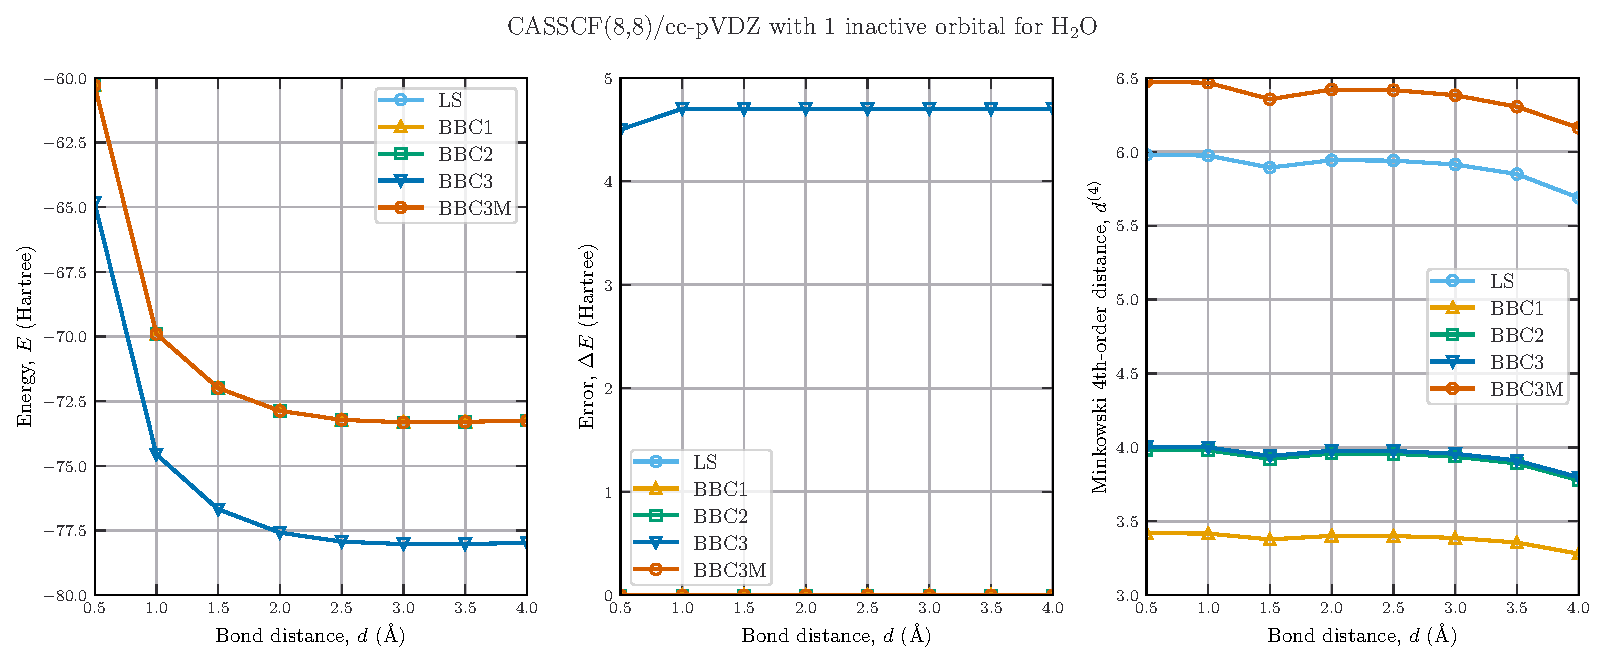
\includegraphics[width=1.0\textwidth]{MCSCF-ccpVDZ.pdf}
        \subimport{figures/}{MCSCF-ccpVDZ.pgf}
        \caption{CASSCF energies, absolute errors and Minkowski distances of order 
        $p=4$ for the LS, BBC1, BBC2, BBC3 and BBC3M approximations.}
        \label{fig:plot_pdf}
    \end{figure}

    This is the result of the main problem discussed in \cref{sec:approximated-Eee},
    the assignment of frontier orbitals.
    In this case, no automatized function was used.
    An orbital $p$ was selected as antibonding if $0 \le n_p \le 0.1$, and as
    bonding if $0.9 \le n_p \le 1$.
    Looking at the results, it can be concluded that this criteria does not perform
    well, but was improved with the modification applied in BBC3M.
    This improvement is noticeable in the third subfigure, where the Minkowski distance
    for BBC3 and BBC3M is noticeable different and, furthermore, the difference
    between BBC2 and BBC3 is not noticeable, meaning that the corrections
    applied to BBC2 leading to BBC3 are not well implemented.
    Also, the BBC3 2-RDM was the only approximated 2-RDM to not fulfill the normalization
    condition, which is a clear indication that important contributions were lost
    with this classification criteria.

    One possible improvement for the classification of bonding and antibonding
    orbitals would be to use the CI coefficients, such that the high-occupation
    orbitals of a relevant configuration (large CI coefficient), associated with
    a decrease of the energy, would be classified as bonding.
    Similarly, a low-occupation orbital of a relevant configuration, associated
    with an increase in the energy, would be classified as antibonding.

    With \cref{tab:minkowski}, and looking at the third subplot of \cref{fig:plot_pdf},
    different values of the Minkowski distance can be observed, eventhough the
    energy errors are very close between all approximations.
    In fact, the Minkowski distance corresponding to BBC3 is lower than that
    corresponding to BBC3M and LS, although the BBC3 approximation is the worst-performing
    approximation.
    This is the main reason why the Minkowski distance is not a performance metric.
    Also, the Minkowski distance for BBC3M is $\sim 4$ times larger than that of
    BBC1, which means that both perform well in this case while being constructed
    differently.

    % Analogous FCI and HF+MP2 calculations have been performed, obtaining very similar
    % results.
    Different order Minkowski distances were computed (see \cref{fig:minkowski-plot}
    in the \cref{sec:appendix-minkowski}), with equivalent results.
    The order $p=4$ is included because, in this case, all distances were
    $0 \le d \le 10$ which is convenient in order to not work with big number.

% ------------------------------
\section{Conclusions and future perspectives} % (fold)
\label{sec:conclusions}
% ------------------------------
In this thesis, the application of Reduced Density Matrix Functional Theory 
(RDMFT) for electronic structure calculations has been extensively explored.
The primary goal was to create a working environment that enables the 
following optimization of the possible new parameterization proposed in this
work.

Several key findings emerged from this study:
\begin{enumerate}[label={}]
    \item \textit{First.} Validation of approximations:
        Stablished approximations for the electron repulsion functional in terms of 
        the two-particle reduced density matrix (2-RDM) have been validated.
        These approximations have shown promise in accurately capturing 
        electron correlation effects in small sized systems, as in this case,
        \ch{H2O}.
    \item \textit{Second.} Possible new parameterization:
        A possible new parameterization of the 2-RDM was proposed, providing 
        possible approaches and algorithms for a future optimization.
    \item \textit{Third.} Computational implementation:
        The methodologies proposed were implemented and tested at
        various theory levels, and is extensible to other systems
        simply changing the Dalton input.
        Their feasibility and effectiveness in practical applications was
        demonstrated.
\end{enumerate}

Reduced Density Matrix Functional Theory presents a promising improvement
in computational cost to wavefunction-based methods.
Therefore, the study of reduced density matrices and their applications
presents multiple avenues for future research.
One of the promising directions is the development of new approximations
and improvement of existing approximations for the electron repulsion functional,
specially for its application to larger systems.

The development of more precise approximated reduced 
density matrices and efficient methods directly repercute in accuratly describing
electronic properties, which has significant implications in fields such as
computational chemistry and solid-state physics. 
% The ability to accurately describe the energy and properties of complex 
% electronic systems can enhance the design of materials and molecules with 
% desired properties, such as more efficient catalysts or materials with 
% specific electronic characteristics

There are a vast of interdisciplinary applications of RDMFT, such as
to molecular biology with the study of quantum-level interactions in biomolecules.
Along those practical applications, RDMFT is used in theoretical physics
to provide new insights into the nature of electronic interactions in strongly
correlated systems.

The principal advantage of using reduced density matrices over classical
wavefunction methods lies in their ability to capture electronic correlation 
without an explicit representation of the 
full many-body wavefunction, which removes exponential grow with the number of 
electrons and orbitals.
The 2-RDM carries all the relevant information if one is interested in
expectation values of one- and two-particle operators, which is almost always
the case.
Therefore, the 2-RDM is a much more compact and economic storage of
information than the $N$-particle wave function.
This reduction in complexity could make such methods computationally feasible
for larger systems and provide a more efficient means of handling electron
correlation effects.
By using functionals of the reduced density matrices, RDMFT can offer a 
balance between accuracy and computational feasibility, making it a powerful 
tool for studying complex electronic systems.

One of the main challenges is that the 2-RDM has to obey complicated
$N$-representability conditions in order to correspond its formal definition
(\cref{eq:sordm-coordinate-representation}), while the wave function only has
to be antisymmetric and normalized to unity.
This results in a high computational complexity problem associated with accurate
approximations of reduced density matrices.
Additionally, one of the main downsides of current methods is their 
application primarily to small systems, for which approximated functionals
have been parametrized.
This limitation arises due to the exponential increase in computational 
resources required as the system size grows, specially for the 2-RDM as it
is constructed as a 4-dimensional tensor.
For larger systems, the computational cost becomes prohibitive because the 
number of possible electronic configurations increases dramatically.

However, with advances in quantum computing and machine learning algorithms,
there is a significant opportunity to overcome these limitations.
For example, the optimization of parametrization factors, such as $\mu$ and
$\mu^{\prime}$ in \cref{eq:AQ-approximation}, with type-algorithms as those
proposed in this work involve expensive methods and algorithms as matrix and
tensor decompositions and diagonalization.
Therefore, the integration of this variational-type methods in quantum computing,
which is a currently developing area, would overcome this problems. 
Also, the integration of machine learning techniques to this kind of 
parametrizations and optimizations could improve the cost and, more importantly,
the application to larger and more complex systems.
% The integration of machine learning techniques could enable the prediction of
% electronic properties more quickly and at a lower computational cost

Over the past few decades, there has been extensive theoretical development 
around reduced density matrices.
This includes the formulation and refinement of the contracted Schrödinger 
equations (CSE), which offer a framework for approximating the many-body 
problem by considering only the RDMs of interest.
% The CSEs have been pivotal in advancing our understanding and computational 
% approaches to electronic correlation in quantum systems.

While this document has primarily focused on the 1-RDM and 2-RDM due to their 
importance, physical significance and relatively simpler formal definitions,
there have been substantial theoretical advancements concerning higher-order
reduced density matrices, such as the 3-RDM and 4-RDM, which are of the most
practical interest.
Also, analogously to the reconstruction of the 1-RDM from the 2-RDM given in
\cref{eq:1rdm-from-2rdm}, lower-order RDMs can be reconstructed from higher-order
ones by tracing over a dimension.
These higher-order RDMs provide even more detailed information about 
electronic interactions but come with increased complexity in both definition 
and computational demand.
Exploring these higher-order RDMs can potentially lead to more accurate 
descriptions of electronic systems and new insights into many-body quantum 
phenomena.

The primary future vision for this work is for the potentially new 
approximation proposed in this document to be verified and optimized. 
By achieving this, the program is intended to be enhanced, generalized, and 
made more efficient, ultimately seeking its possible integration with existing 
software such as Dalton.

Additionally, since no time-dependence has been considered in this work, 
an important extension would be the development and application to Time-Dependent
Reduced Density Matrix Functional Theory (TDRDMFT), which is a relatively 
young extension of RDMFT and represent a significant future research direction.
TDRDMFT can provide insights into the dynamic behavior of 
electronic systems under various external perturbations, enhancing our 
understanding of time-dependent processes in complex quantum systems with
the advantage of RDMFT.

Looking forward, several future research directions have been identified:
\begin{itemize}
    \item Time-Dependent Extensions:
        Extending the current methodologies to Time-Dependent Reduced Density 
        Matrix Functional Theory (TDRDMFT) could provide valuable insights 
        into dynamic processes in electronic systems.
    \item Theoretical Advancements:
        Optimization of the proposed parametrization and testing.
    \item Integration with Existing Software:
        Integration of the program with existing software such as Dalton.
\end{itemize}

In conclusion, this thesis provides a comprehensive framework for employing 
reduced density matrice in electronic structure calculations, highlighting both
its potential and the challenges that need to be addressed.
The field of Reduced Density Matrix Functional Theory and RDM approximations is
full of opportunities and challenges.
It is essential to continue improving existing 
approximations and methodologies and exploring new techniques that can overcome current limitations.
With the convergence of different disciplines and the use of emerging 
technologies, the future of this field promises to be exciting and full of 
innovative discoveries.
The advancements made here lay the groundwork for further study of the possible
new approximation proposed in this work, and for future studies in the theory.


% =============================================================================
%                             --- References ---
% =============================================================================
% \newpage
% \addcontentsline{toc}{section}{Bibliografía}
\clearpage
% \renewcommand{\thesection}{} % Elimina la numeración de secciones
\begin{singlespace}
    % \bibliographystyle{achemso}
    \printbibliography[title={References}] % change from bibliography to references
    \addcontentsline{toc}{section}{References}
\end{singlespace}
% =============================================================================
%                             --- Appendix ---
% =============================================================================
\clearpage
% ------
\section{Appendix}
\label{sec:appendix}
% ------

\lstinputlisting[
    language=bash,
    % firstline=2,
    % lastline=12,
    label={lst:CASSCF-input},
    caption={Dalton input file for the CASSCF(8,8) with 1 inactive orbital
    calculations for \ch{H2O}.}
]{data/DALTON.INP}

\end{document}
%%%%%%%%%%%%%%%%%%%%%%%%%%%%%%%%%%%%%%%%%%%%%%%%%%%%%%%%%%%%%%%%%%%%%%%%%%%%%%%
